\clearpage
\gdef\ztexKeyValParent{}
\subsection{\titlepkg{sect} 模块}
\subsubsection{序言}\label{sect:intro}
\zTeX{} 的 \pkg{sect} 模块重写了与章节和目录相关的所有命令, 其提供了一系列的命令和接口用于章节和目录的自定义; 该模块的实现
参考了 \pkg{ctex-headings}, \pkg{titlesec}, \pkg{titletoc}, \pkg{etoc} 以及 \CusTeX, C\TeX{} 两个宏集; 但 \pkg{sect} 模块并
不依赖于以上的任意一个宏包或宏集. 在介绍此模块提供命令前, 我们做如下的约定:

\pkg{sect} 模块中将章节标题(\texttt{title}) 分为 ``\texttt{num, name}'' 两个部分, 比如 ``\texttt{1.1 foo}'' 中 
``\texttt{num = 1.1}'', ``\texttt{name = foo}''; 
为后续行文方便, 我们在章节标题相关的上下文中:  称 ``\texttt{title}'' 为 ``\textbf{标题}'', 
称 ``\texttt{num}'' 为 ``\textbf{编号}'', 称 ``\texttt{name}'' 为 ``\textbf{名称}''.

\pkg{sect} 模块中将章节目录分为
``\texttt{name, title, leader, page}'' 四个部分, 比如 ``\texttt{1.2 bar ... 1}'' 中 
``\texttt{name = 1.2}'', ``\texttt{title = bar}'', ``\texttt{leader=...}'', ``\texttt{page = 1}''.
为后续行文方便, 我们在目录相关的上下文中: 称 ``\texttt{name}'' 为 ``\textbf{名称}''; 
称 ``\texttt{title}'' 为 ``\textbf{标题}'', 称 ``\texttt{leader}'' 为 ``\textbf{引导线}'',
称 ``\texttt{page}'' 为 ``\textbf{页码}''. 后文的 ``(章节)目录, 表格目录, 图片目录, ...''
我们统称为 ``\texttt{table}''.


\pkg{sect} 模块会阻止 \pkg{titlesec}, \pkg{titletoc} 等宏包的加载; 也就是说, 
当用户加载 \pkg{sect} 模块后, 便不能再加载 \pkg{titlesec}, \pkg{titletoc}, \pkg{etoc} 等宏包了,
它们与本模块中的部分设置冲突.

\pkg{sect} 模块并不包含类似 \pkg{titlesec} 宏包所提供的那些标题样式，比如 \texttt{wrap}、\texttt{leftmargin}、
\texttt{drop} 等. 但是它们都可以通过 ``\texttt{explicit}'' 选项来实现, 比如: 结合 \cs{hangindent}、
\cs{hangafter} 以及 ``\texttt{explicit}'' 选项, 我们就可以轻松实现 ``wrap'' 样式.


\vskip2em
\noindent{\sffamily\color{red}NOTE: 
\begin{enumerate}
  \item \pkg{sect} 模块还处于早期开发阶段, 很多的功能还不够完善:比如 Tagged PDF, 术语(glossary)和索引支持等.
  \item \pkg{sect} 模块和 \pkg{ctex} 宏包中 heading 相关的设置相冲突.
  \item \pkg{sect} 模块和 \ztex{} 中的部分模块或库目前处于耦合状态, 请慎用 ``\texttt{sect/load=false}'' 设置.
  \item \pkg{sect} 模块中和 glossary 相关的命令和变量暂时不要使用, 会有一些潜在的问题: 比如其对应的数据文件为 \texttt{\string\jobname.log}，这会和编译的日志文件相冲突(目前已经将其临时更改为 \texttt{tog(table of glossary)}).
\end{enumerate}}


\clearpage
\subsubsection{层级/模板}
\ztex{} 支持动态创建标题, 以及标题层级重定义. \ztex{} 会自动处理 Mark, Bookmark 和目录等内容. 
除此之外, 本节还收录了部分命令用于修改章节命令或目录模板.


\begin{function}[added=2025-08-30]{\zseclevelmap}
  \begin{syntax}
    \cs{zseclevelmap}\Arg{keyval}
  \end{syntax}
  此命令用于调整当前文档的标题层级或新增标题层级, 只能在导言区使用. \meta{keyval} 中的 ``键'' 为标题/目录类型, 比如
  ``\texttt{chapter}, \texttt{section}, \texttt{figure}, \texttt{table}'' 等; \meta{keyval}
  中的 ``值'' 为一个整数, 代表该标题/目录类型的层级, 可以为负数. \textbf{备注}: 在声明一个新的标题层级后, 用户还需要使用
  \cmd{\zsecdefine} 命令定义该命令的一些必要参数后才能在后续使用此标题层级. 为了让新的标题层级能够在目录中正常排版, 用户
  还需要建立其对应的目录(模板)实例, 参见 \cmd{\zsecdefine} 命令中的说明.
\end{function}


\begin{function}[added=2025-09-08]{\zsecTemplateDefaultsEdit}
  \begin{syntax}
  \cs{zsecTemplateDefaultsEdit}\Arg{keyval}
  \end{syntax}
  此命令用于修改 \pkg{sect} 模块中标题模板的默认值. \meta{keyval} 的可用键值列表
  请参见: \cref{sect:keyval}. \textbf{备注}: 此命令对已经创建实例的章节命令无效.
\end{function}



\clearpage
\subsubsection{章节标题}\label{sect:keyval}
\begin{keyval}{explicit, code}
  \begin{syntax}
    explicit = \meta{true|\textbf{false}} > \dval{false}
    code     = \meta{code} > \dval{空}
  \end{syntax}
  \meta{explicit} 键与 \pkg{titlesec} 宏包的 ``\texttt{explicit}'' 选项类似, 但在 
  \pkg{sect} 模块中, 用户可以仅对部分章节命令启用该选项; 当 ``\texttt{explicit = true}'' 
  时, 用户需要在 \meta{code} 中指定该章节标题的内容; 此时需借助 \cmd{\zsecnum}, \cmd{\zsecname}, \cmd{\zsecclass} 等宏.
  \vskip.5em\relax
  \noindent{\sffamily\color{red}NOTE:普通用户不建议使用 `\texttt{explicit}' 键，因为此时需要用户手动处理目录和书签等内容; 为了照顾另一部分用户, 这里给出处理目录和书签需要用到的两个内部函数:\cmd{\__zsect_title_toc_add:nnn}, \cmd{\__zsect_bookmark_update:nnn}. 这两个命令的参数格式一致, 默认情况下: 第一个参数为 \cmd{\zsecclass}, 第二个参数为 \cmd{\zsectocname}, 第三个参数为 \cmd{\zsecname}. }
\end{keyval}


\begin{function}[updated=2026-02-15, EXP]{
    \zsecclass,
    \zsecname,
    \zsectocname,
    \zsecnum,
    \zsectocnum, 
    \zsectocHnum
  }
  在 ``\texttt{explicit}'' 的 \meta{code} 或 \cmd{\zsecformat} 中, 可以使用 ``\cs{zsecclass}'' 表示当前的类型, 
  使用 ``\cs{zsecnum}'' 表示 \meta{num} 对应的内容, 使用 ``\cs{zsecname}'' 表示 \meta{name} 对应的内容, 使用 \cmd{\zsectocname} 
  表示当前章节命令写入目录条目对应的 ``title(标题)'' 值; \cmd{\zsectocnum} 表示当前章节命令写入目录条目的 ``name(名称)'' 值;
  \cmd{\zsectocHnum} 表示当前章节命令写入目录条目的超链接目标索引. 一个简单的设置案例如下:\par
  \noindent \textbf{注意}:用户可以在 ``\texttt{explicit}'' 的 \meta{code} 或 \cmd{\zsecformat} 中使用这些命令;
  但在这些地方之外, 这些命令输出的内容无任何实际意义或不可用; 当用户重定义 \cmd{\thesection} 等宏时, \cmd{\zsecnum}
  等宏会同步进行更改(修改 \cmd{\theHsection} 等宏时也同理).
\end{function}
\vskip1.25em\relax
\begin{DocExample}
\zsecformat{\section, \subsection,}
  {
    explicit=true, 
    code={(\zsecclass){\color{blue}\zsecnum}:[\zsecname]\par}
  }
\end{DocExample}



\begin{keyval}{type, pagestyle}
  \begin{syntax}
    type        = \meta{page|top|normal} > \dval{空}
    pagestyle   = \meta{style} > \dval{空}
  \end{syntax}
  \meta{type} 用于指定该类型章节命令的排版方式: 占据整页(\texttt{page}), 
  位于页面顶端(\texttt{top}), 普通样式(\texttt{normal}); \meta{pagestyle} 用于指定该类型章节标题所在页面的
  页面格式, 一般只针对 \meta{type} 为 ``\texttt{page, top}'' 的章节命令.
\end{keyval}


\begin{keyval}{hang, break, afterindent}
  \begin{syntax}
    hang        = \meta{true|\textbf{true}} > \dval{true}
    break       = \meta{code} > \dval{空}
    afterindent = \meta{true|\textbf{false}} > \dval{false}
  \end{syntax}
  \meta{hang} 用于指定该类型章节命令的长标题是否需要悬挂缩进; \meta{break} 用于控制标题所在位置的分页, 普通用户
  可以忽略该选项; \meta{afterindent} 用于指定该类型章节命令后的第一个段落是否首行缩进.
  {\sffamily\color{red} ``break'' 键暂时不可用.}
\end{keyval}



\begin{keyval}{space.before, space.after, space.left}
  \begin{syntax}
    space.before = \Arg{skip} > \dval{空}
    space.after  = \Arg{skip} > \dval{不定}
    space.left   = \Arg{length} > \dval{空}
  \end{syntax}
  \meta{space.before} 用于设置标题前的垂直间距; \meta{space.after} 用于设置标题后的垂直间距,
  若 \texttt{title.inline = true}, 则该距离会被转为水平距离; \meta{space.left} 用于设置标题的左侧距离.
\end{keyval}



\begin{keyval}{title.inline, title.format, title.format+, title.before, title.after}
  \begin{syntax}
    title.inline  = \meta{true|\textbf{false}} > \dval{false}
    title.format  = \meta{code} > \dval{空}
    title.format+ = \meta{code} > \dval{空}
    title.before  = \meta{code} > \dval{空}
    title.after   = \meta{code} > \dval{\char92par}
  \end{syntax}
  \meta{title.inline} 用于控制标题是否换行, 会影响 \meta{space.before}, \meta{space.after} 
  的作用方式(详情请参见后两者说明); \meta{title.format} 和 \meta{title.format+} 会同时作用于
  ``编号'' 和 ``名称'', 前者会覆盖原有的样式, 后者会将新的格式代码加入原样式; \meta{title.before}
  置于 ``标题'' 前, 位于 \meta{num.before} 之前; \meta{title.after} 置于 ``标题'' 后, 位于 
  \meta{name.after}(以及 \meta{name.sep}) 之后.
\end{keyval}


\begin{keyval}{num, num.show, num.sep, num.width, num.format, num.format+, num.before, num.after}
  \begin{syntax}
    num         = \meta{code} > \dval{空}
    num.show    = \meta{\textbf{true}|false} > \dval{true}
    num.sep     = \meta{length} > \dval{空}
    num.width   = \meta{length} > \dval{空}
    num.format  = \meta{code} > \dval{空}
    num.format+ = \meta{code} > \dval{空}
    num.before  = \meta{code} > \dval{空}
    num.after   = \meta{code} > \dval{空}
  \end{syntax}
  \meta{num} 用于指定标题编号, 若为空, 则使用 ``\cs{the\meta{class}}'' 的默认值;
  \meta{num.show} 控制这里的所有键, 当 ``\texttt{num.show = true}'' 时, 这些键才有意义;
  \meta{num.sep} 用于指定标题编号后的额外间距; \meta{num.width} 用于指定标题编号宽度,
  默认为空, 此时该选项无效(该项常应用于一些较宽编号); \meta{num.format}
  用于指定标题编号格式, 会覆盖原有格式; \meta{num.format+} 会将新的格式代码加入原代码,
  不会覆盖原有格式, 且编号内容可以被格式代码最后的含参命令捕获; \meta{num.before} 用于向编号前添加内容;
  \meta{num.before} 会向其后添加内容; \par\vskip.5em\relax
  \noindent{\color{red}\sffamily NOTE: \ztex{} 的 \pkg{sect} 模块同时考虑了键 \meta{num.show}(, 目录中的 \meta{name.show}) 和计数器 ``\texttt{secnumdepth}'', ``\texttt{tocdepth}'', 三者均会影响 ``编号(名称)'' 的显示; 不同的是: \meta{num.show} 仅影响标题排版时是否显示 ``编号'', 对目录文件没有影响; 与之类似的, 目录设置中的 \meta{name.show} 只影响目录在排版时是否显示 ``名称''; 但计数器 ``\texttt{secnumdepth}'' 和 ``\texttt{tocdepth}'' 会同时影响标题文本和目录文件, 前者会影响 ``编号'' 的写入, 后者用于决定是否将该层级的章节命令写入目录文件.}
\end{keyval}


\begin{keyval}{name.sep, name.format, name.format+, name.before, name.after}
  \begin{syntax}
    name.sep     = \meta{length} > \dval{空}
    name.format  = \meta{code} > \dval{空}
    name.format+ = \meta{code} > \dval{空}
    name.before  = \meta{code} > \dval{空}
    name.after   = \meta{code} > \dval{空}
  \end{syntax}
  \meta{name.sep} 用于指定标题名称后的额外间距; \meta{name.format}
  用于指定标题名称格式, 会覆盖原有格式; \meta{name.format+} 会将新的格式代码加入原代码,
  不会覆盖原有格式, 且名称内容可以被格式代码最后的含参命令捕获; \meta{name.before} 用于向名称前添加内容;
  \meta{name.before} 会向其后添加内容.
\end{keyval}


\begin{keyval}{format.num, format.num+, format.name, format.name+, format.title, format.title+}
  \begin{syntax}
    format       = \meta{code} > \dval{空}
    format+      = \meta{code} > \dval{空}
    num.format   = \meta{code} > \dval{空}
    num.format+  = \meta{code} > \dval{空}
    name.format  = \meta{code} > \dval{空}
    name.format+ = \meta{code} > \dval{空}
  \end{syntax}
  \meta{format.num} 同 \meta{num.format};
  \meta{format.num+} 同 \meta{num.format+}; 
  \meta{format.name} 同 \meta{name.format}; 
  \meta{format.name+} 同 \meta{name.format+}; 
  \meta{format.title} 同 \meta{title.format}; 
  \meta{format.title+} 同 \meta{title.format+}.
\end{keyval}


\begin{keyval}{bookmark.num, bookmark.cmd, bookmark.before, bookmark.after}
  \begin{syntax}
    bookmark.num    = \meta{true|\textbf{false}} > \dval{false}
    bookmark.cmd    = \meta{function} > \dval{\texttt{\#1:->\#1}}
    bookmark.before = \meta{code} > \dval{空}
    bookmark.after  = \meta{code} > \dval{空}
  \end{syntax}
  这两个键用于指定书签中该章节命令对应 \meta{name} 的前后内容. \meta{bookmark.num} 
  为 \texttt{true} 时将显示书签前的编号. \meta{function} 用于自定义书签的样式, 其接受一个
  参数, 表示当前的书签内容. 关于 \meta{bookmark.cmd}, 一个简单的使用样例如下(两种方法效果一样):
\end{keyval}
\vskip1em\relax
\begin{DocExample}
%% wrap bookmark content in '()' for '\section' 
%  and '\subsection' classes.
% method I:
\def\TTTa#1{(#1)}
\zsecformat{\section, \subsection}{bookmark.cmd=\TTTa{##1}}
% method II:
\zsecformat{\section, \subsection}{bookmark.cmd=(##1)}
\end{DocExample}



\clearpage
\begin{function}[added=2025-09-10]{\zsectitlestyle}
  \begin{syntax}
    \cs{zsectitlestyle}\Arg{style}
  \end{syntax}
  \meta{style} 用于指定新建立的章节命令所属的\textbf{样式}, 
  仅能在导言区使用. \pkg{sect} 模块中章节命令的默认样式为 ``\texttt{ltx}'',
  用户可以使用后续的 \cmd{\zsecdefine} 命令自定义章节命令主题.
\end{function}


\begin{function}[added=2025-09-08]{\zsectitleOnce}
  \begin{syntax}
  \cs{zsectitleOnce}\Arg{class}\Arg{keyval}\oarg{toc-content}\Arg{sec-content}
  \cs{zsectitleOnce}*\Arg{class}\Arg{keyval}\oarg{toc-content}\Arg{sec-content}
  \end{syntax}
  此命令用于排版一次性的标题, 不会影响其它标题格式. \meta{class} 用于指定此章节命令的层级;
  \meta{keyval} 用于指定标题的属性, 可用的键值列表请参见: \cref{sect:keyval}; \meta{toc-content} 
  用于指定目录中的内容, 若为空, 此时目录中的该条目使用 \meta{sec-content}; \meta{sec-content} 
  用于指定标题内容. \cmd{\zsectitleOnce*} 用于排版无编号标题, \textbf{不会}写入目录.
\end{function}



\begin{function}[added=2025-08-29]{\zsecdefine}
  \begin{syntax}
    \cs{zsecdefine}\meta{class}\Arg{style}\Arg{keyval}
  \end{syntax}
  此命令封装自 \cs{zsect_define_title:Nnn} 命令, 用于自定义章节命令格式; 
  \meta{style} 用于指定新建立的章节命令所属的样式; \meta{keyval} 中所有的可用键值列表参见节首说明. 
  \meta{class} 可以是 ``\verb|\part, \section, \subsection, ...|'' 等. 
  \textbf{备注}: 如果该 \meta{class} 目录条目的 instance 不存在, 那么用户需手动指定, 参见下面的示例;\par
  % \noindent{\color{red}\sffamily NOTE: \meta{keyval} 中必须指明 ``\texttt{class}'' 键对应的值.}
\end{function}
\begin{DocExample}[++]
% note: create a new class 'book' of level 0, but
%       instance 'ztoc/level0' does not exsit.
\zseclevelmap{book=0}
\DeclareInstance{ztextoc}{ztoc/level0}{default}
  {
    format         = \large\bfseries\color{red},
    name.width     = 1.9em,
    space.before   = 1em\@plus\p@,
    space.hang     = 1.9em,
    space.left     = 1.9em,
    leader.content = ,
  }
\end{DocExample}


\begin{function}[updated=2025-09-08]{\zsecformat}
  \begin{syntax}
    \cs{zsecformat}\oarg{style}\Arg{classes}\Arg{keyval}
    \cs{zsecformat}*\oarg{style}\Arg{classes}\Arg{keyval}
  \end{syntax}
  此命令用于设置类型为 \meta{classes} 的章节命令格式. \meta{style} 用于指定新建立的章节命令所属的样式,
  默认值为 ``\texttt{ltx}''; \meta{classes} 可以是 ``\verb|\part|, \verb|\section, \subsection|'' 等; 
  \meta{keyval} 用于设置其属性; 带有 ``\texttt{*}'' 的命令用于设置无编号标题的格式(是指 \verb|\chapter*{}, \section*{}|
  这样的命令, 而非自身就无编号的 \verb|\paragraph{} 或 \subparagraph{}| 命令). \vskip1em
  \noindent{\color{red}\sffamily NOTE: 该命令的作用是局部的.}
\end{function}



\begin{function}[added=2025-09-07, updated=2025-09-10]{\zseccaption}
  \begin{syntax}
    \cmd{\zseccaption}\Arg{class}\oarg{format}\Arg{content}
  \end{syntax}
  此命令用于手动添加 caption(即使不在浮动体环境中), 且它会调用 \cs{zsect_add_\meta{class}_line:eeee} 进行目录的添加. 
  \meta{class} 可选值有 ``\texttt{figure, table, theorem, lstlisting, algorithm, glossary}''; \meta{format} 用于自定义
  caption 的格式, 在 \meta{format} 中, 使用 \verb|#1| 表示其前缀(形如 ``\texttt{Figure \meta{num}}''), 使用 \verb|#2| 
  表示 caption 的内容, 默认值为 ``\verb|#1\IfBlankF{#2}{:}#2|''; \meta{content} 为 caption 的内容, \ztex{} 会自动为其增加前缀: \cs{fnum@\meta{class}}. 
  (当 \meta{content} 为空时, 中间的冒号 -- ``\texttt{:}'' 不会显示)\par
  \noindent \textbf{备注}: \meta{class} 不能为 ``\texttt{toc}''; 此命令封装自后续的 \cmd{\zsect_caption_use:nnn} 命令; \meta{content} 中的脆弱命令可以不用保护.
\end{function}



\clearpage
\subsubsection{章节目录}\label{ss2:toc}
当目录相关的变量改变或目录数据有更新时, 请编译文档至少两次, 以得到正确的结果.

\vskip.5em\relax
\noindent{\color{red}\sffamily NOTE: toc 相关设置会覆盖 \pkg{hyperref} 中 \texttt{linkcolor} 的设定, 前者优先级更高.}

\begin{keyval}{explicit, enhance, code}
  \begin{syntax}
    explicit = \meta{true|\textbf{false}} > \dval{false}
    enhance  = \meta{true|\textbf{false}} > \dval{false}
    code     = \meta{code} > \dval{空}
  \end{syntax}
  \meta{explicit} 键与 \pkg{titlesec} 宏包的 ``\texttt{explicit}'' 选项类似, 但在 
  \pkg{sect} 模块中, 用户可以仅对部分章节命令启用该选项; \meta{enhance} 设置为 ``\texttt{true}''
  后, 会启用 \cmd{\ztocthehilevel}, \cmd{\ztocthecard} 等高级宏; 当 ``\texttt{explicit = true}'' 
  时, 用户需要在 \meta{code} 中指定该章节标题的内容; 此时用户需借助 \cmd{\ztocdepth}, 
  \cmd{\ztocname}, \cmd{\ztoctitle} 和 \cmd{\ztocpage} 命令, 它们的作用描述如下:
\end{keyval}


\begin{function}[updated=2025-09-19, EXP]{
    \ztocclass, \ztocstyle, \ztocdepth, \ztocname, 
    \ztoctitle, \ztocpage, \ztocanchor
  }
  \begin{syntax}
  \cmd{\ztocclass}
  ...
  \cmd{\ztocanchor}
  \end{syntax}
  这些宏可以在 ``\texttt{explicit}'' 的 \meta{code} 或 \cmd{\ztocformat} 命令中使用: 
  \cs{ztocclass} 表示当前的目录的类型, ``\texttt{section, chapter}'' 等; \cs{ztocstyle} 表示当前目录的样式, 有编号/无编号;
  使用 ``\cs{ztocdepth}'' 表示当前的目录条目的深度; 使用 ``\cs{ztocname}'' 表示当前目录条目 \meta{name} 中的内容;
  使用 ``\cs{ztoctitle}'' 表示当前目录条目 \meta{title} 中的内容; 使用 ``\cs{ztocpage}'' 表示当前目录条目的页码. 
  \cs{ztocanchor} 表示目录条目对应其在文档中的 link target.
  % \textbf{备注}:除 \cmd{\ztoclink} 外, 其余的命令均可以在 \texttt{e}-型参数中被完全展开.
  \par \noindent \textbf{备注}: 与前述章节命令里 ``\texttt{explicit}'' 选项相同: 用户可以在 ``\texttt{explicit}'' 
  的 \meta{code} 或 \cmd{\ztocformat} 命令内部使用这些它们(比如在 \meta{title.after} 键中使用), 但在这些地方之外, 
  这些命令输出的内容无任何实际意义或不可用.
\end{function}


\begin{function}[updated=2025-09-19]{\ztoclink}
  \begin{syntax}
    \cmd{\ztoclink}\Arg{text}
  \end{syntax}
  这个宏可以在 ``\texttt{explicit}'' 的 \meta{code} 或 \cmd{\ztocformat} 命令中使用, 用于创建超链接文本.
  \textbf{备注}: 在这些地方之外, 此命令的输出内容无实际意义或不可用.
\end{function}


\begin{function}[updated=2025-09-19, EXP]{\ztocifnumbered}
  \begin{syntax}
    \cmd{\ztocifnumbered}\Arg{true code}\Arg{false code}
  \end{syntax}
  这个宏可以在 ``\texttt{explicit}'' 的 \meta{code} 或 \cmd{\ztocformat} 命令中使用, \cmd{\ztocifnumbered}
  用于测试当前条目是否含有编号, 含有编号执行 \meta{true code}(\meta{name.show} 对此命令没有影响). 
  \textbf{备注}: 在这些地方之外, 此命令的输出内容无实际意义或不可用.
\end{function}


\begin{function}[updated=2025-09-18, rEXP]{
    \ztoctheindex, \ztoctheabsindex, \ztocthecard,
    \ztocthehilevel, \ztocthelolevel,
  }
  当 ``\texttt{enhance = true}'' 时, 这些命令才有效, 且\textbf{只能}在 ``\texttt{explicit}'' 
  的 \meta{code} 中使用. \cs{ztoctheindex} 表示当前目录的\textbf{相对索引}; \cs{ztoctheabsindex} 表示当
  前目录的\textbf{绝对索引}; \cs{ztocthecard} 表示当前目录所包含的子目录数量; \cs{ztocthehilevel} 
  和 \cs{ztocthelolevel} 分别表示当前所排版目录中 \meta{class} 的最小值与最大值. \textbf{备注}: 
  这些高级宏启用后, 文档编译会花费更多的时间.
\end{function}

一个简单的目录格式设置案例如下:\par
\vskip1em\relax
\begin{DocExample}
\ztocformat{\subsection, \subsubsection}
  { explicit = true,
    code = {
      \hskip2em\rule[1pt]{5pt}{5pt}~
        {\bfseries \ztocname}~\hb@xt@5\ccwd{\ztoctitle}~
      \fbox{\hyper@link{link}{page.\ztocpage}{\ztocpage}}\par
    }
  }
\end{DocExample}


\begin{keyval}{no-parent}
  \begin{syntax}
    no-parent  = \meta{true|\textbf{false}} > \dval{false}
  \end{syntax}
  若该键设置为 ``\texttt{true}'', 则当前目录的父级条目会被隐藏; 
  {\color{red}\sffamily ``no-parent'' 键暂时不可用}
\end{keyval}


\setlength{\dvalwidth}{6em}
\begin{keyval}{line.end, line.width}
  \begin{syntax}
    line.end   = \meta{code}> \dval{\string\ztoc@line@end}
    line.width = \meta{length} > \dval{空}
  \end{syntax}
  \meta{line.end} 用于控制每个目录条目结束时的行为, 默认为 \cs{ztoc@line@end}, 该宏默认定义为 
  \cs{par}; \meta{line.width} 用于指定当前目录条目的宽度, 该键在处理较长的目录条目时很有用.
  {\color{red}\sffamily ``line.width'' 键暂时不可用}
\end{keyval}


\begin{keyval}{space.before, space.left, space.right, space.hang}
  \begin{syntax}
    space.before = \meta{skip} > \dval{空}
    space.left   = \meta{skip} > \dval{空}
    space.right  = \meta{skip} > \dval{\string\ztoc@rmargin}
    space.hang   = \meta{length} > \dval{空}
  \end{syntax}
  \meta{space.before} 表示该目录条目前面的垂直间距; \cmd{\ztoc@rmargin} 默认
  为 \cmd{\@tocrmarg}; 后面几个长度的含义请参见如下图示(此图截取自 \CusTeX{} 宏集手册):\vskip1em
  \centerline{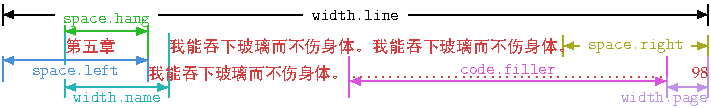
\includegraphics{./support/pics/toc_shape.pdf}}
\end{keyval}
\setlength{\dvalWidth}{2.25em}
\setlength{\dvalwidth}{2em}


\begin{keyval}{width.name, width.title, width.page, width.line}
  这几个长度的含义请参见上面的图示(该图截取自 \CusTeX{} 宏集手册);
  \meta{width.name} 同 \meta{name.width};
  \meta{width.title} 同 \meta{title.width};
  \meta{width.page} 同 \meta{page.width};
  {\color{red}\sffamily ``width.title, width.line'' 键暂时不可用}
\end{keyval}


\begin{keyval}{name, name.show, name.width, name.hyper, name.format, name.format+, name.before, name.after}
  \begin{syntax}
    name         = \meta{code} > \dval{空}
    name.show    = \meta{\textbf{true}|false} > \dval{true}
    name.width   = \meta{length} > \dval{空}
    name.hyper   = \meta{true|\textbf{false}} > \dval{false}
    name.format  = \meta{code} > \dval{空}
    name.format+ = \meta{code} > \dval{空}
    name.before  = \meta{code} > \dval{空}
    name.after   = \meta{code} > \dval{空}
  \end{syntax}
  \meta{name} 用于指定目录条目的编号, 若为空, 则使用当前的 ``名称''; \meta{name.show} 用于指定是否显示目录条目``名称''(编号),
  若为 ``\texttt{true}'', 则显示; \meta{name.width} 用于指定名称对应的宽度, 当 \texttt{\meta{name.width} = 0pt} 时, 
  将使用 ``名称'' 的自然宽度; \meta{name.hyper} 用于设置名称是否启用超链接; \meta{name.format} 用于指定目录条目名称的格式, 
  会覆盖原有的格式; \meta{name.format+} 会将新的格式代码加入原代码, 不会覆盖原有的格式, 且名称内容可以被格式代码最后的含参命令捕获;
  \meta{name.before} 用于向名称前添加内容; \meta{name.before} 用于向名称后添加内容;\vskip1em 
  \noindent{\color{red}\sffamily NOTE: \ztex{} 的 \pkg{sect} 模块同时考虑了键 \meta{num.show}(, 目录中的 \meta{name.show}) 和计数器 ``\texttt{secnumdepth}'', ``\texttt{tocdepth}'', 三者均会影响 ``编号(名称)'' 的显示; 不同的是: \meta{num.show} 仅影响标题排版时是否显示 ``编号'', 对目录文件没有影响; 与之类似的, 目录设置中的 \meta{name.show} 只影响目录在排版时是否显示 ``名称''; 但计数器 ``\texttt{secnumdepth}'' 和 ``\texttt{tocdepth}'' 会同时影响标题文本和目录文件, 前者会影响 ``编号'' 的写入, 后者用于决定是否将该层级的章节命令写入目录文件.}
\end{keyval}


\begin{keyval}{title.hyper, title.format, title.format+, title.before, title.after}
  \begin{syntax}
    title.hyper   = \meta{true|\textbf{false}} > \dval{false}
    title.format  = \meta{code} > \dval{空}
    title.format+ = \meta{code} > \dval{空}
    title.before  = \meta{code} > \dval{空}
    title.after   = \meta{code} > \dval{空}
  \end{syntax}
  \meta{title.hyper} 用于设置标题是否启用超链接; \meta{title.format}
  用于指定标题的格式, 会覆盖原有的格式; \meta{title.format+} 会将新的格式代码加入原代码,
  不会覆盖原有的格式, 且标题内容可以被格式代码最后的含参命令捕获; \meta{title.before} 用于向标题前添加内容; 
  \meta{title.after} 用于向标题后添加内容; {\color{red}\sffamily ``title.width'' 键暂时不可用}
\end{keyval}


\begin{keyval}{hyper.name, hyper.title, hyper.page}
  \meta{hyper.name} 同 \meta{name.hyper};
  \meta{hyper.title} 同 \meta{title.hyper}; 
  \meta{hyper.page} \\ 同 \meta{page.hyper}; 
\end{keyval}


\setlength{\dvalWidth}{3.5em}
\setlength{\dvalwidth}{6em}
\begin{keyval}{leader.fill, leader.sep, leader.raise, leader.type, leader.content}
  \begin{syntax}
    leader.fill    = \meta{skip} > \dval{\string\hfill}
    leader.sep     = \meta{length} > \dval{\string\ztoc@leader@sep}
    leader.raise   = \meta{length} > \dval{\string\ztoc@leader@raise}
    leader.type    = \meta{\meta{空}|x|c|} > \dval{\string\ztoc@leader@type}
    leader.content = \meta{token} > \dval{\string\ztoc@leader@content}
  \end{syntax}
  这一系列的键用于控制目录中 ``引导线'' 的样式; 它们可以单独设置, 也可以通过设置
  \cs{ztoc@leader@sep}, \cs{ztoc@leader@raise} 等宏进行全局设置; \meta{leader.fill}
  用于设置整个引导线的宽度, 默认为 \cs{fill};
  \cs{ztoc@leader@sep} 默认为 ``\texttt{4.6pt}'', \cs{ztoc@leader@raise} 默认为 
  ``\texttt{0pt}'', \cs{ztoc@leader@type} 默认为 ``\texttt{\meta{空}}'', 
  \cs{ztoc@leader@content} 默认为 ``\texttt{.}''.
\end{keyval}



\begin{keyval}{page.width, page.hyper, page.format, page.format+, page.before, page.after}
  \begin{syntax}
    page.width   = \meta{length} > \dval{\string\ztoc@page@width}
    page.hyper   = \meta{true|\textbf{false}} > \dval{false}
    page.format  = \meta{code} > \dval{\string\normalfont\string\normalcolor}
    page.format+ = \meta{code} > \dval{空}
    page.before  = \meta{code} > \dval{空}
    page.after   = \meta{code} > \dval{空}
  \end{syntax}
  \meta{page.width} 用于设置页码的宽度. \meta{page.hyper} 用于设置页码是否启用超链接; 
  \meta{page.format} 用于指定页码格式, 会覆盖原有的格式, 默认值为 \verb|\normalfont\normalcolor|; \meta{page.format+} 会将新的格式代码加入原代码,
  不会覆盖原有的格式, 且页码内容可以被格式代码最后的含参命令捕获; \meta{page.before} 用于向名称前添加内容;
  \meta{page.before} 用于向名称后添加内容;
\end{keyval}
\setlength{\dvalWidth}{2.25em}
\setlength{\dvalwidth}{2em}


\setlength{\dvalWidth}{2.25em}
\setlength{\dvalwidth}{7.5em}
\begin{keyval}{ignore, ignore.negate, ignore.name, ignore.text, ignore.page}
  \begin{syntax}
    ignore        = \meta{true|\textbf{false}} > \dval{false}
    ignore.negate = \meta{true|\textbf{false}} > \dval{false}
    ignore.name   = \meta{clist} > \dval{\string\s__ztoc_ignore_empty_mark}
    ignore.text   = \meta{tl} > \dval{空}
    ignore.page   = \meta{clist} > \dval{空}
  \end{syntax}
  这一系列键用于忽略特定的目录条目, 满足除 \meta{ignore.negate} 以外任何一个条件的
  目录条目将会被忽略; \meta{ignore} 为 ``\texttt{true}'' 时表示
  忽略该条目, 反之, 则保留; 若当前目录条目的 \meta{name} 包含于 \meta{ignore.name} 
  这个逗号分割列表中, 则该目录条目会被忽略; 若当前目录条目的 \meta{title} 中包含有 \meta{ignore.text} 
  内的关键词, 则该目录条目会被忽略; 若当前目录条目的 \meta{page} 包含于 \meta{ignore.page} 
  中, 则该目录条目会被忽略; \meta{ignore.negate} 表示将上述的操作反向, 即, 只\textbf{保留}满足这些 ``忽略条件''
  的项目.
\end{keyval}
\vskip1.25em\relax
\noindent{\color{red}\sffamily NOTE:
  \begin{enumerate}\setlength{\itemsep}{0pt}\setlength{\parskip}{0pt}
    \item 当 \meta{ignore.negate} 为 ``\texttt{true}'' 时, \ztex{} 会依次去判断这些 ``忽略条件'', 当找到满足条件
          的一个目录条目后, 余下的 ``忽略条件'' 将会被跳过;
    \item 在进行比较时, \meta{ignore.name} 或 \meta{ignore.text} 不需要将匹配内容写完整, 二者均支持部分匹配; 比如目录中
          的部分 \meta{title} 为 ``\texttt{AAA-1, AAA-2}'', 那么用户只需要指定 \meta{ignore.text}\texttt{ = AAA} 
          即可匹配上述的两个 \meta{title}.
    \item 这里的比较是基于字符串本身的, 且控制序列后的空格在比较时会被忽略. 比如 ``\verb|\ztocformat\subsection{ignore.name={\textbf{T}\;}}|'', 
          这个设置将会忽略如下的目录条目:
          \def\exampleUR{}
          \begin{DocExample}
          \contentsline{subsection}{{\textbf {T}\;}{XXX}}{YYY}{ZZZ}%
          \end{DocExample}
          \resetExampleUR
  \end{enumerate}
}\par\noindent
我们以后续的定理目录数据作为案例展示 ``\texttt{ignore}'' 相关键的作用:
\begin{DocExample}*
{
  % select subsection with '\textbf {L}\;'
  \ztocformat\subsection
    {
      ignore.negate=true, 
      ignore.name={\textbf {L}\;}
    }
  \ztocformat\section{ignore=true} % ignore all section
  \zthmtoc
}
\end{DocExample}
\setlength{\dvalWidth}{2.25em}
\setlength{\dvalwidth}{2em}



\begin{keyval}{
  format, format+, 
  format.name, format.name+, 
  format.title, format.title+,
  format.page, format.page+,
  }
  \meta{format} 用于控制当前目录条目中 \meta{name}, \meta{title} 和 \meta{page} 的格式; \meta{format+} 
  作用和前者作用相同, 但其仅会追加到已有的格式代码中; \textbf{备注}: \meta{format.page} 的默认值为 \verb|\normalfont\normalcolor|. 
  \meta{format.name} 同 \meta{name.format};
  \meta{format.name+} 同 \meta{name.format+};
  \meta{format.title} 同 \meta{title.format};\\
  \meta{format.title+} 同 \meta{title.format+}; 
  \meta{format.page} 同 \meta{page.format};\\ 
  \meta{format.page+} 同 \meta{page.format+}; 
\end{keyval}


\begin{function}[updated=2025-07-06]{\ztocenable}
  \begin{syntax}
    \cs{ztocenable}\oarg{keyval}
  \end{syntax}
  此命令用于启用目录功能, 在导言区添加此命令后 \cs{tableofcontents}, \cs{ztocenable} 等命令才能正常使用;
  \meta{keyval} 用于设置目录类型与来源, 默认值为 \verb|toc|, 其中可同时填入多个值, 使用逗号分割; 每一项的格式
  为 ``\meta{type} = \meta{file}'', \meta{type} 的可选值有 ``\texttt{toc, lof, lot, lom, log, loa}'', \meta{file} 
  为对应的文件名(不需要添加后缀), 且 \meta{file} 可以省略, 默认的文件名为 \cs{jobname}, 该文件的后缀为默认的 \meta{key} 
  值. 比如 ``\cs{ztocenable}\texttt{\{lom\}}'', 它会启用 ``定理目录(lom)'', 其依赖的目录文件为 ``\cs{jobname}\texttt{.lom}''.
  % \par
  % \textbf{注意}: 由于后续的 \cs{zlocaltoc} 命令依赖于 ``\texttt{*.ptoc}'' 文件, 当用户需要自定义局部目录的文件源时,
  % 请提供对应的 ``\texttt{*.ptoc}'' 文件, 否则 \cs{zlocaltoc} 输出内容为空. ``\texttt{ptoc}'' 文件的格式可参考本节
  % 末测试用例.
\end{function}


\begin{function}[added=2025-09-08]{\ztoclineOnce}
  \begin{syntax}
    \cs{ztoclineOnce}\Arg{keyval}\Arg{class}\{\Arg{name}\Arg{title}\}\Arg{page}
  \end{syntax}
  此命令用于排版一次性的目录, 不会影响其它目录条目. \meta{keyval} 的可用键值列表请参见: \cref{ss2:toc};
  \meta{class} 的可选值有 ``\texttt{section, chapter, figure, theorem, ...}'' 等; \meta{name}, \meta{title}
  和 \meta{page} 的含义在本节已经做过说明, 这里不在复述.
\end{function}


\begin{function}[added=2025-09-08]{\ztocTemplateDefaultsEdit}
  \begin{syntax}
  \cs{ztocTemplateDefaultsEdit}\Arg{keyval}
  \end{syntax}
  此命令用于修改 \pkg{sect} 模块中目录模板的默认值. \meta{keyval} 的可用键值列表
  请参见: \cref{ss2:toc}. \textbf{备注}: 此命令对已经创建实例的目录命令无效.
\end{function}


\begin{function}[updated=2025-07-06]{\tableofcontents}
  \begin{syntax}
    \cs{tableofcontents}\oarg{file}
  \end{syntax}
  此命令用于输出文档的全部目录, 当 \cs{ztocenable} 启用目录后可用; 和 \Hologo{LaTeX2e} 中 \cs{tableofcontents} 命令
  不同的是: 该命令可以在文档中任意位置，任意次数使用; \meta{file} 用于指定目录对应的 ``\texttt{*.toc}'' 文件,
  \textbf{不需要}添加文件后缀, 默认为 \verb|\jobname|.
\end{function}


\begin{function}[updated=2025-07-06]{\multicolcontents}
  \begin{syntax}
    \cs{multicolcontents}\oarg{file}\marg{column}
  \end{syntax}
  此命令将使用多栏布局输出文档的全部目录; \meta{file} 用于指定目录对应的 ``\texttt{*.toc}'' 文件,
  \textbf{不需要}添加文件后缀, 默认为 \verb|\jobname|. \meta{column} 表示目录栏数, 接受一个整数.
\end{function}


\begin{function}[added=2025-09-04]{\ztocstop}
  \begin{syntax}
  \cs{ztocstop}\oarg{tables}
  \end{syntax}
  此命令会停止目录的收集, 它之后的所有目录数据均不会被记录, 用户应慎用此命令.
  \meta{tables} 为一个逗号分割列表, 默认为 ``\texttt{toc}''.
\end{function}


\begin{function}[added=2025-07-10]{\ztocset}
  \begin{syntax}
    \cs{zlocaltoc}\Arg{keyval}
  \end{syntax}
  此命令用于设置目录的格式, 它将作用于所有的目录层级; 可用的键值列表参见下面的说明:
\end{function}


\ExplSyntaxOn
\gdef\ztexKeyValParent{\zkeycolor{gray}{\l__codedoc_parent_key_ztex_tl/}}
\ExplSyntaxOff
\begin{keyval}[parent=ztex/ztoc/option]{
  rmargin, ignore.level, line.end, page.width,
  leader.type, leader.sep, leader.raise, leader.content
  }
  这些键的具体含义在前文已经做过说明，这里不再重复.
\end{keyval}
\ExplSyntaxOn
\gdef\ztexKeyValParent{}
\ExplSyntaxOff


\begin{function}[updated=2025-09-11]{\zlocaltoc}
  \begin{syntax}
    \cs{zlocaltoc}\oarg{file}\Arg{class}\Arg{index list}
  \end{syntax}
  此命令用于输出局部目录, 可以在文章中的任意地方, 任意次数使用. \meta{file} 用于指定目录对应的 ``\texttt{*.toc}'' 文件,
  \textbf{不需要}添加文件后缀, 默认为 \verb|\jobname|; \meta{index list} 为一个逗号分割列表, 其中的每一个元素为一个
  整数 \meta{index}, 表示 \meta{class} 在目录文中的\textbf{相对索引}; 此命令用于输出第 \meta{index} 个 \meta{class} 
  及其包含的所有子目录. \meta{class} 可以是 ``\texttt{part, section, subsection, figure, table}'' 等; \meta{index} 从 1 
  开始计数. \par 
  \textbf{注意}: \fbox{1.} \meta{index} 并不是 ``\texttt{*.ptoc}'' 文件中 ``\texttt{name}'' 后面的值; 举个例子: 
  比如 \texttt{*.ptoc} 文件中有这么一行内容 ``\verb|class={subsection}, name={1.3}, ...|'', 
  假如该行的前面还有 4 行含有 \texttt{subsection}(不管它们嵌套在哪个层级中), 此时用户需要
  将 \meta{index} 置为 ``5''. \fbox{2.} \cs{zlocaltoc} 命令能够利用 ``\texttt{class, name, title, page, raw}''
  所有字段的值, 可以参见命令: \cmd{\ztoc_table_filter_key_byclass:nnnNN}; \fbox{3.} 如果用户不希望手动计算 \meta{class}
  的\textbf{相对索引}, 可以使用后续的 \cmd{\ztocindex} 命令, 其会根据 \meta{class} 和 \meta{title} 自动返回 \textbf{相对索引}.
  % \fbox{3.} 当用户需要自定义局部目录的文件源时,
  % 请提供对应的 ``\texttt{*.ptoc}'' 文件(通过前述的 \cs{ztocenable} 命令进行设置), 否则 \cs{zlocaltoc} 输出内容为空.
  \vskip2em
  \noindent {\sffamily\color{red}NOTE: 该命令将得到的结果(一系列的 \cs{contentsline}) 保存于 \texttt{\char92g_ztoc_local\meta{table}_seq}
  这个 seq 中, \meta{table} 取决于用户指定的 \meta{class}, 用户可以按照自己的方式操作此 seq.}
\end{function}
\begin{DocExample}*
{
  \ztocformat\subsection{title.after=\P}
  \zlocaltoc{section}{2}
}
\end{DocExample}


\begin{function}[added=2025-07-08]{\ztocgroupshow, \ztocgrouphide}
  \cs{ztocgroupshow} 命令用于显示局部目录中的插入点(Hook), 当用户无法确定 \cs{ztocgroupinsert} 命令中的 
  \meta{place} 时, 此命令是十分有用的; \cs{ztocgrouphide} 用于隐藏这些插入点. \vskip1em
  \noindent{\color{red}\sffamily NOTE: 这两个命令的作用是局部的.}  
\end{function}
\begin{DocExample}*
{
  \ztocgroupshow
  \zlocaltoc{subsection}{5}
}
\end{DocExample}


\begin{function}[added=2025-07-30]{ztoc/tocline/begin, ztoc/tocline/end}
  在 \ztex{} 中, 每条目录的前后放置了这两个钩子; 一般的钩子机制请参见后续的 \cmd{\ztocgroupinsert}
  命令.
\end{function}


\begin{function}[added=2025-07-07]{\ztocgroupinsert}
  \begin{syntax}
    \cs{ztocgroupinsert}\Arg{place}\Arg{code}
  \end{syntax}
  \pkg{sect} 模块对目录进行了分组, 并且在每组目录的前后都放置了一个 Hook(这些 Hook 是根据当前的文档内容动态生成的), 
  用户可以向这些 Hook 中添加代码(这些添加进去的代码都是一次性的), 从而实现目录的进一步定制; \meta{place} 为 Hook 的名字, 其格式为:
  ``\meta{class},\meta{index},\meta{before|begin|end|after}'', 它们的位置关系请参见: \cref{ztoc:hook-position}; 其中 \meta{index} 的计算方法和 \cs{zlocaltoc} 命令中 \meta{index}
  的计算方法\textbf{不同}, 前者(\verb|\ztocgroupinsert| 命令中的 \meta{index})只需考虑当前局部环境内该 \meta{class} 
  的次序; \par\vskip1.25em\relax
  \noindent{\color{red}\sffamily NOTE: 如果当前的排版的目录为空, 那么 \meta{code} 可能会插入到之后目录的 hooks 中.}
\end{function}
\par\vskip1.25em\relax


下面这个示例展示了该命令的基本使用方法, 文件 ``\texttt{./support/data/data.toc}'' 的内容请
参见: \cref{outer-toc:custom_file}.
\par\vskip1.25em\relax

\begin{DocExample}*[++]
\ztocgroupinsert{subsection,1,begin}{{\fbox{T1-BEGIN}}}
\ztocgroupinsert{subsection,1,end}{{\fbox{T1-END}}\par}
\ztocgroupinsert{subsection,2,begin}{{\fbox{T2-BEGIN}}}
\ztocgroupinsert{subsection,2,end}{{\fbox{T2-END}}\par}
\ztocformat\subsection{space.before=.5em}
\ztocformat\subsubsection
  {
    explicit = true,
    code = \fcolorbox{red}{gray}{\ztoctitle}\-,
  }
\zlocaltoc[./support/data/data]{section}{1}
\end{DocExample}
% \ExplSyntaxOn
% \seq_show:c {g_ztoc_toc_seq}
% \seq_show:c {g_ztoc_keyvaltoc_seq}
% \ExplSyntaxOff

% 由于此处的命令 \verb|\ztocenable| 会改变之后所有与目录相关的变量, 所以在这里我们直接插入运行结果图:
% \vskip1em\relax
% \noindent\fbox{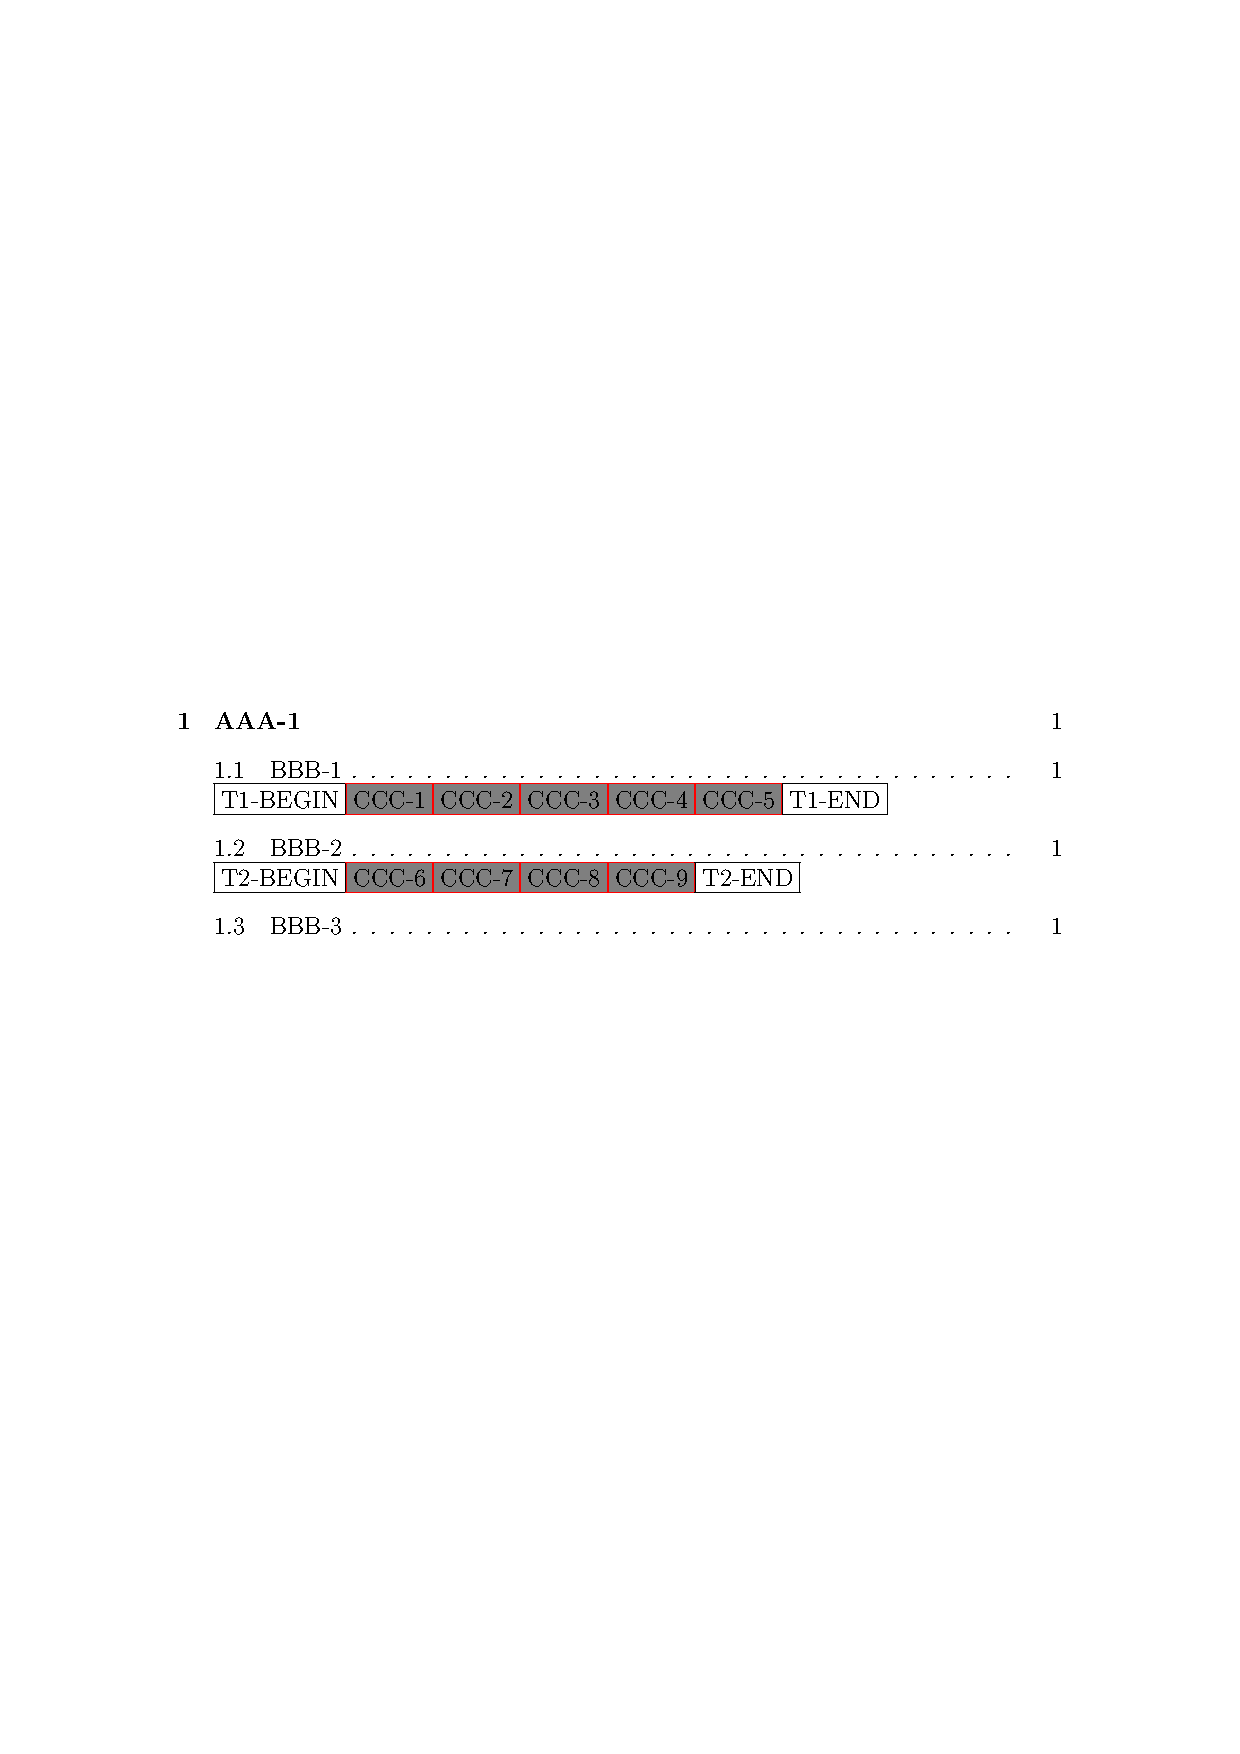
\includegraphics[width=\textwidth]{./support/pics/toc_group_example2.pdf}}


\begin{function}[updated=2025-07-06]{\ztocformat}
  \begin{syntax}
    \cs{ztocformat}\Arg{classes}\Arg{keyval}
  \end{syntax}
  此命令用于设置类型为 \meta{classes} 的章节命令格式, \meta{classes} 可以是
  ``\verb|\part|, \verb|\section, \subsection, figure, table|'' 等; \meta{keyval} 用于设置其属性.
  \vskip1em
  \noindent{\color{red}\sffamily NOTE: 该命令的作用是局部的.}
\end{function}
\begin{DocExample}*
\makeatletter{
  \ztocformat\subsection 
    { explicit = true,
      code = {
        \noindent {\bfseries \ztocname~ \ztoctitle}
        \cleaders\hbox{.}\hfill\ztocpage\par
    }}
  \ztocformat\subsubsection
    { explicit = true,
      code = {
        \hskip2em\rule[1pt]{5pt}{5pt}~{\bfseries \ztocname}~\hb@xt@5\ccwd{\ztoctitle}~
        \fbox{\hyper@link{link}{page.\ztocpage}{\ztocpage}}\par
    }}
  \zlocaltoc{subsection}{\ztocindex{subsection}{\pkg{font} 模块}}
}\makeatother
\end{DocExample}


\begin{function}[added=2025-09-10]{\ztocotherformat}
  \begin{syntax}
    \cs{ztocotherformat}\oarg{class}\Arg{keyval}
  \end{syntax}
  此命令用于定义除 ``\texttt{toc}'' 外的其它目录样式. \meta{class} 用于指定设置的目录对象,
  可选值有: ``\texttt{figure, table, theorem, lstlisting, algorithm, glossary}'', 默认值为 ``\texttt{figure}'';
  \meta{keyval} 格式请参见:\cref{ss2:toc}. \textbf{备注}: 该命令也可以使用上述的 \cs{ztocformat} 命令替代.
\end{function}



\begin{function}[added=2025-09-12, EXP]{\ztocslot}
  \begin{syntax}
  \cmd{\ztocslot}
  \end{syntax}
  此命令返回当前目录条目在当前目录层级中对应的序号, 这个值总是有意义的.
\end{function}



\begin{function}[added=2025-09-18, rEXP]{\ztoccard}
  \begin{syntax}
  \cmd{\ztoccard}\oarg{table}\Arg{class}\Arg{title}
  \end{syntax}
  此命令返回由 \meta{class} 和 \meta{title} 所确定目录的\textbf{子}目录(card 即 cardinality),
  如果由 \meta{class} 和 \meta{title} 所确定目标目录不存在, 其返回 ``-1''; \meta{table} 用于指定
  当前所排版目录对应的 keyval seq 变量, 可选值有: ``\texttt{toc, lot, ...}'' 等.
\end{function}



\begin{function}[added=2025-09-18, rEXP]{\ztochilevel, \ztoclolevel}
  \begin{syntax}
    \cmd{\ztochilevel}\marg{table}
    \cmd{\ztoclolevel}\marg{table}
  \end{syntax}
  这两个命令会返回 \meta{seq} 中的 class level 数据, \meta{seq} 为目录对应
  的 keyval seq 变量: \texttt{\char92 g_ztoc_keyval\meta{table}\_seq}.
  \meta{seq} 由 \meta{table} 指定, \meta{table} 的可选值有 ``\texttt{toc, lot, lof}'' 等.
  \cmd{\ztochilevel} 返回 \meta{seq} 中最小的 level 值; \cmd{\ztoclolevel} 返回 \meta{seq} 
  中最大的 level 值; \textbf{备注}: \meta{class} 级别越高, 对应的 level 值越小.
\end{function}



\begin{function}[added=2025-09-12, rEXP]{\ztocindex}
  \begin{syntax}
  \cmd{\ztocindex}\oarg{table}\Arg{class}\Arg{title}
  \cmd{\ztocindex*}\oarg{table}\Arg{class}\Arg{title}
  \end{syntax}
  命令 \cmd{\ztocindex} 用于返回由 \meta{class} 和 \meta{title} 所确定条目在
  seq 变量 \texttt{\char92 g_ztoc_keyval\meta{table}_seq} 中的相对索引, 
  \cmd{\ztocindex*} 返回绝对索引(不考虑目录的 \meta{class} 值). \meta{table} 用于指定当前所排版目录
  对应的 keyval seq 变量, 可选值有: ``\texttt{toc, lot, ...}'' 等. 
  \textbf{备注}: 如果没有满足筛选条件的目录, 此命令总是返回一个小于零的整数值.
  \vskip1.25em\relax
  \noindent{\sffamily\color{red}NOTE: \meta{class} 和 \meta{title} 比较的是字符串本身, 而不是 token 的比较;
  所以部分情况下, 用户需要将它们二者提前展开.}
\end{function}



\begin{function}[added=2025-09-12, EXP]{\ztociffirst}
  \begin{syntax}
    \cmd{\ztociffirst}\Arg{true code}\Arg{false code}
  \end{syntax}
  此命令和 \pkg{etoc} 宏包提供的 \cmd{\tociffirst} 作用相同, 用于判断当前的目录是否为其所在的 level 
  的第一项. 此命令在 \meta{code} 选项中十分有用, 其用法可以参见: \cref{toc-longtable} 中的案例.
  \textbf{备注}: 在 \texttt{e/f}-type 中, 此命令\textbf{可以}被完全展开;
\end{function}


\begin{function}[added=2025-09-13, rEXP]{\ztocifmiddle}
  \begin{syntax}
  \cs{ztocifmiddle}\oarg{table}\Arg{true code}\Arg{false code}
  \end{syntax}
  此命令用于判断当前目录条目是否位于两条同级目录之间. \meta{table} 默认为 \texttt{toc}.
  \textbf{备注}:实际上是判断当前目录条目之后的条目是否为同级目录.
\end{function}


\begin{function}[added=2025-09-12, rEXP]{\ztociflast}
  \begin{syntax}
  \cmd{\ztociflast}\oarg{table}\Arg{true code}\Arg{false code}
  \end{syntax}
  此命令用于判断当前目录是否为其所在 level 的最后一项. \meta{table} 用于指定当前所排版目录
  对应的 keyval seq 变量, 可选值有: ``\texttt{toc, lot, ...}'' 等. 
  \textbf{备注}: 实际上是判断当前目录条目之后的条目是否为更高一级的目录(例如 section 比 subsection 的级别更高);
  在 \texttt{e}-type 中, 此命令\textbf{能}被完全展开.
  \vskip1.25em\relax
  \noindent{\sffamily\color{red}NOTE: 当最后的目录条目为
  ``\verb|\contentsline{subsection}{}{}{}|, \\
  \verb|\contentsline{subsection}{}{}{}|'' 时, 此命令对于上述 ``\texttt{section}'' 条目的判断会出错, 
  此时用户可以手动添加对应的代码.}
\end{function}


下面这个例子说明了 \ztex{} 在目录中不同位置时，对 \texttt{first}、\texttt{middle}、\texttt{last} 
的判断方式:
\begin{DocExample}*[++]
\begingroup\ExplSyntaxOn
\ztocformat{\section, \subsection, \subsubsection}
  {
    page.before=
      {
        % uncoment the following line:
        % \typeout{---->expandable:[\ztociflast{Yes}{No}]}
        {\color{red}(First:\ztociffirst{Yes}{No})}|
        {\color{blue}(Middle:\ztocifmiddle{Yes}{No})}|
        {\color{purple}(Last:\ztociflast{Yes}{No})}|
      },
    leader.content={},
  }
\ExplSyntaxOff
\tableofcontents[./support/data/data_II]
\endgroup
\end{DocExample}



\begin{function}[added=2025-09-15, updated=2025-09-19]{\ztocgroupparser}
  \begin{syntax}
    \cmd{\ztocgroupparser}
    ~~~~\oarg{table}\oarg{step code}\Arg{cmd}
    ~~~~\Arg{before}\Arg{begin}\Arg{end}\Arg{after}
  \end{syntax}
  此命令用于格式化目录数据, 格式化后的数据保存于 \cmd{\ztocgroupparserOutput} 变量中. 
  \meta{table} 默认值为 ``\texttt{toc}''; \meta{step code} 在每一条目录处理完成后执行, 可以置为空.
  \textbf{备注}: 此命令封装自后续的 \cmd{\ztoc_group_parser:NNNnnnnn} 命令, 使用方法请参见
  后者的说明.
\end{function}


\begin{function}[added=2025-09-15, EXP]{
    \gparserclass,
    \gparserindex,
    \gparseranchor,
  }
  这些变量可以在 \cmd{\ztoc_group_parser:NNNnnnnn} 或 \cmd{\ztocgroupparser} 中使用, 它们在写入 \meta{tl}
  时会被执行 \texttt{e}-型展开, 所以请将脆弱命令使用 \cmd{\noexpand} 或 \cmd{\unexpanded} 保护起来.
  \textbf{备注}: 在 \cmd{\ztoc_group_parser:NNNnnnnn} 或 \cmd{\ztocgroupparser} 命令之外, 这些变量不可用或包含错误的值.
\end{function}



\begin{function}[added=2025-09-06]{
    \listoffigures,
    \listoftables,
    \listoftheorems,
    \listoflistings,
    \listofalgorithoms,
    \printglossaries,
    \listofglossaries,
  }
  这系列命令用于输出图片目录, 表格目录, 定理目录 ...,  可以在正文中多次使用; 
  当 ``\texttt{lof, lot, lom, ...}'' 启用后才可用, 且它们不接受任何参数; 
  \textbf{注意}: 重定义 \cs{listfigurename}, \cs{listtablename} 等宏 
  没有作用, 用户需手动添加章节命令; \cmd{\printglossaries} 和 \cmd{\listofglossaries}
  为同一个命令.
  \vskip1.25em\relax
  \noindent{\sffamily\color{red}NOTE: 和 glossary 相关的命令暂时不要使用, 它们还未完全适配.}
\end{function}
\begin{DocExample}*
\listoftables
\end{DocExample}



\newgeometry{left=2.5cm, right=2.5cm}
\subsubsection{使用案例}\label{outer-toc:custom_file}
最后附上一些复杂的目录格式定制示例, 涵盖目录样式设置以及目录数据提取, 可作为用户深度定制的参考. 下面这段代码展示了后续样例会用
到的一些命令和依赖宏包:

\begin{dxample}[1]
% \usepackage{tikz}
% \usepackage{tikz-qtree}
% \usepackage[log]{tikz-qtree-patch}
% \usetikzlibrary { mindmap, trees }
\definecolor{SeaGreen}{rgb}{0.18, 0.55, 0.34}
\def\customtocthemecolor{SeaGreen}
\ExplSyntaxOn\makeatletter
\dim_new:N \linewidthfix
\def\tocupdatelinewidthfix{
  \dim_set:Nn \linewidthfix {\linewidth-2\fboxsep}
}
\def\ornamentcorner#1#2#3{
  \node[anchor=#1, rotate=#3, outer~sep=0pt, inner~sep=0pt] at (frame.#2)
  {\pgfornamenthan[width=.8cm, color=\customtocthemecolor]{10}};}
\def\ztochyperpage#1{\exp_args:Nne \hyper@link{link}{page.#1}{#1}}
\makeatother\ExplSyntaxOff
\end{dxample}



\paragraph{测试数据}\label{ztoc-example-data} 本手册在排版目录时用到的测试数据: ``\texttt{data.toc}'', ``\texttt{data\_II.toc}'', ``\texttt{data.ptoc}''. \texttt{data.ptoc} 文件仅用于向读者展示 \pkg{sect} 模块中 keyval seq 的存储结构； 当 ``\texttt{dump-ptable = true}'' 时,
\ztex{} 会自动生成该文件.

\def\exampleUR{\texttt{data.toc}}
\begin{DocExample}[++]
\contentsline {section}{{1}{AAA-1}}{1}{}
\contentsline {subsection}{{1.1}{BBB-1}}{1}{}
\contentsline {subsubsection}{{1.1.1}{CCC-1}}{1}{}
\contentsline {subsubsection}{{1.1.2}{CCC-2}}{1}{}
\contentsline {subsubsection}{{1.1.3}{CCC-3}}{1}{}
\contentsline {subsubsection}{{1.1.4}{CCC-4}}{1}{}
\contentsline {subsubsection}{{1.1.5}{CCC-5}}{1}{}
\contentsline {subsection}{{1.2}{BBB-2}}{1}{}
\contentsline {subsubsection}{{1.2.1}{CCC-6}}{1}{}
\contentsline {subsubsection}{{1.2.2}{CCC-7}}{1}{}
\contentsline {subsubsection}{{1.2.3}{CCC-8}}{1}{}
\contentsline {subsubsection}{{1.2.4}{CCC-9}}{1}{}
\contentsline {subsection}{{1.3}{BBB-3}}{1}{}
\end{DocExample}


\def\exampleUR{\texttt{data\_II.toc}}
\begin{DocExample}[++]
\contentsline{section}{{1}{AAA-1}}{1}{}%
\contentsline{subsection}{{1}{BBB-1}}{1}{}%
\contentsline{subsubsection}{{1.1.1}{CCC-1}}{1}{}%
\contentsline{subsubsection}{{1.1.2}{CCC-2}}{2}{}%
\contentsline{subsubsection}{{1.1.3}{CCxxxC-3}}{3}{}%
\contentsline{subsubsection}{{1.1.4}{CCssgda\-shgfeC-4}}{100}{}%
\contentsline{subsubsection}{{1.1.5}{CsasfCC-5}}{123}{}%
\contentsline{subsubsection}{{1.1.6}{CasklklCC-x}}{999}{}%
\contentsline{subsection}{{2}{B   BB-2}}{1}{}%
\contentsline{subsubsection}{{1.2.1}{CCC-6}}{1}{}%
\end{DocExample}


\def\exampleUR{\texttt{data.ptoc}}
\begin{DocExample}[++]
class={section},name={1},title={AAA-1},page={1},anchor={section.1},raw={\contentsline {section}{{1}{AAA-1}}{1}{}}
class={subsection},name={1.1},title={BBB-1},page={1},anchor={subsection.1.1},raw={\contentsline {subsection}{{1.1}{BBB-1}}{1}{}}
class={subsubsection},name={1.1.1},title={CCC-1},page={1},anchor={subsubsection.1.1.1},raw={\contentsline {subsubsection}{{1.1.1}{CCC-1}}{1}{}}
class={subsubsection},name={1.1.2},title={CCC-2},page={1},anchor={subsubsection.1.1.2},raw={\contentsline {subsubsection}{{1.1.2}{CCC-2}}{1}{}}
class={subsubsection},name={1.1.3},title={CCC-3},page={1},anchor={subsubsection.1.1.3},raw={\contentsline {subsubsection}{{1.1.3}{CCC-3}}{1}{}}
class={subsubsection},name={1.1.4},title={CCC-4},page={1},anchor={subsubsection.1.1.4},raw={\contentsline {subsubsection}{{1.1.4}{CCC-4}}{1}{}}
class={subsubsection},name={1.1.5},title={CCC-5},page={1},anchor={subsubsection.1.1.5},raw={\contentsline {subsubsection}{{1.1.5}{CCC-5}}{1}{}}
class={subsection},name={1.2},title={BBB-2},page={1},anchor={subsection.1.2},raw={\contentsline {subsection}{{1.2}{BBB-2}}{1}{}}
class={subsubsection},name={1.2.1},title={CCC-6},page={1},anchor={subsubsection.1.2.1},raw={\contentsline {subsubsection}{{1.2.1}{CCC-6}}{1}{}}
class={subsubsection},name={1.2.2},title={CCC-7},page={1},anchor={subsubsection.1.2.2},raw={\contentsline {subsubsection}{{1.2.2}{CCC-7}}{1}{}}
class={subsubsection},name={1.2.3},title={CCC-8},page={1},anchor={subsubsection.1.2.3},raw={\contentsline {subsubsection}{{1.2.3}{CCC-8}}{1}{}}
class={subsubsection},name={1.2.4},title={CCC-9},page={1},anchor={subsubsection.1.2.4},raw={\contentsline {subsubsection}{{1.2.4}{CCC-9}}{1}{}}
class={subsection},name={1.3},title={BBB-3},page={1},anchor={subsection.1.3},raw={\contentsline {subsection}{{1.3}{BBB-3}}{1}{}}
\end{DocExample}
\resetExampleUR



\clearpage
\paragraph{案例:1} 一个很简单的案例:

\begin{DocExample}*
\begingroup
\ztocformat\subsection
  {
    format+=\color{teal}, 
    leader.sep=1pt, 
    leader.raise=2.5pt, 
    page.width=10pt
  }
\ztocgroupinsert{subsection,1,begin}%
  {%
    \begin{framed}%
    \pgfornament[width = 2cm,color = teal]{67}%
    \qquad\rule[-5em]{.5pt}{10em}%
    \begin{minipage}{.75\linewidth}%
  }
\ztocgroupinsert{subsection,1,end}%
  {%
    \end{minipage}%
    \end{framed}%
  }
\zlocaltoc{subsection}{4}
\endgroup
\end{DocExample}

% \noindent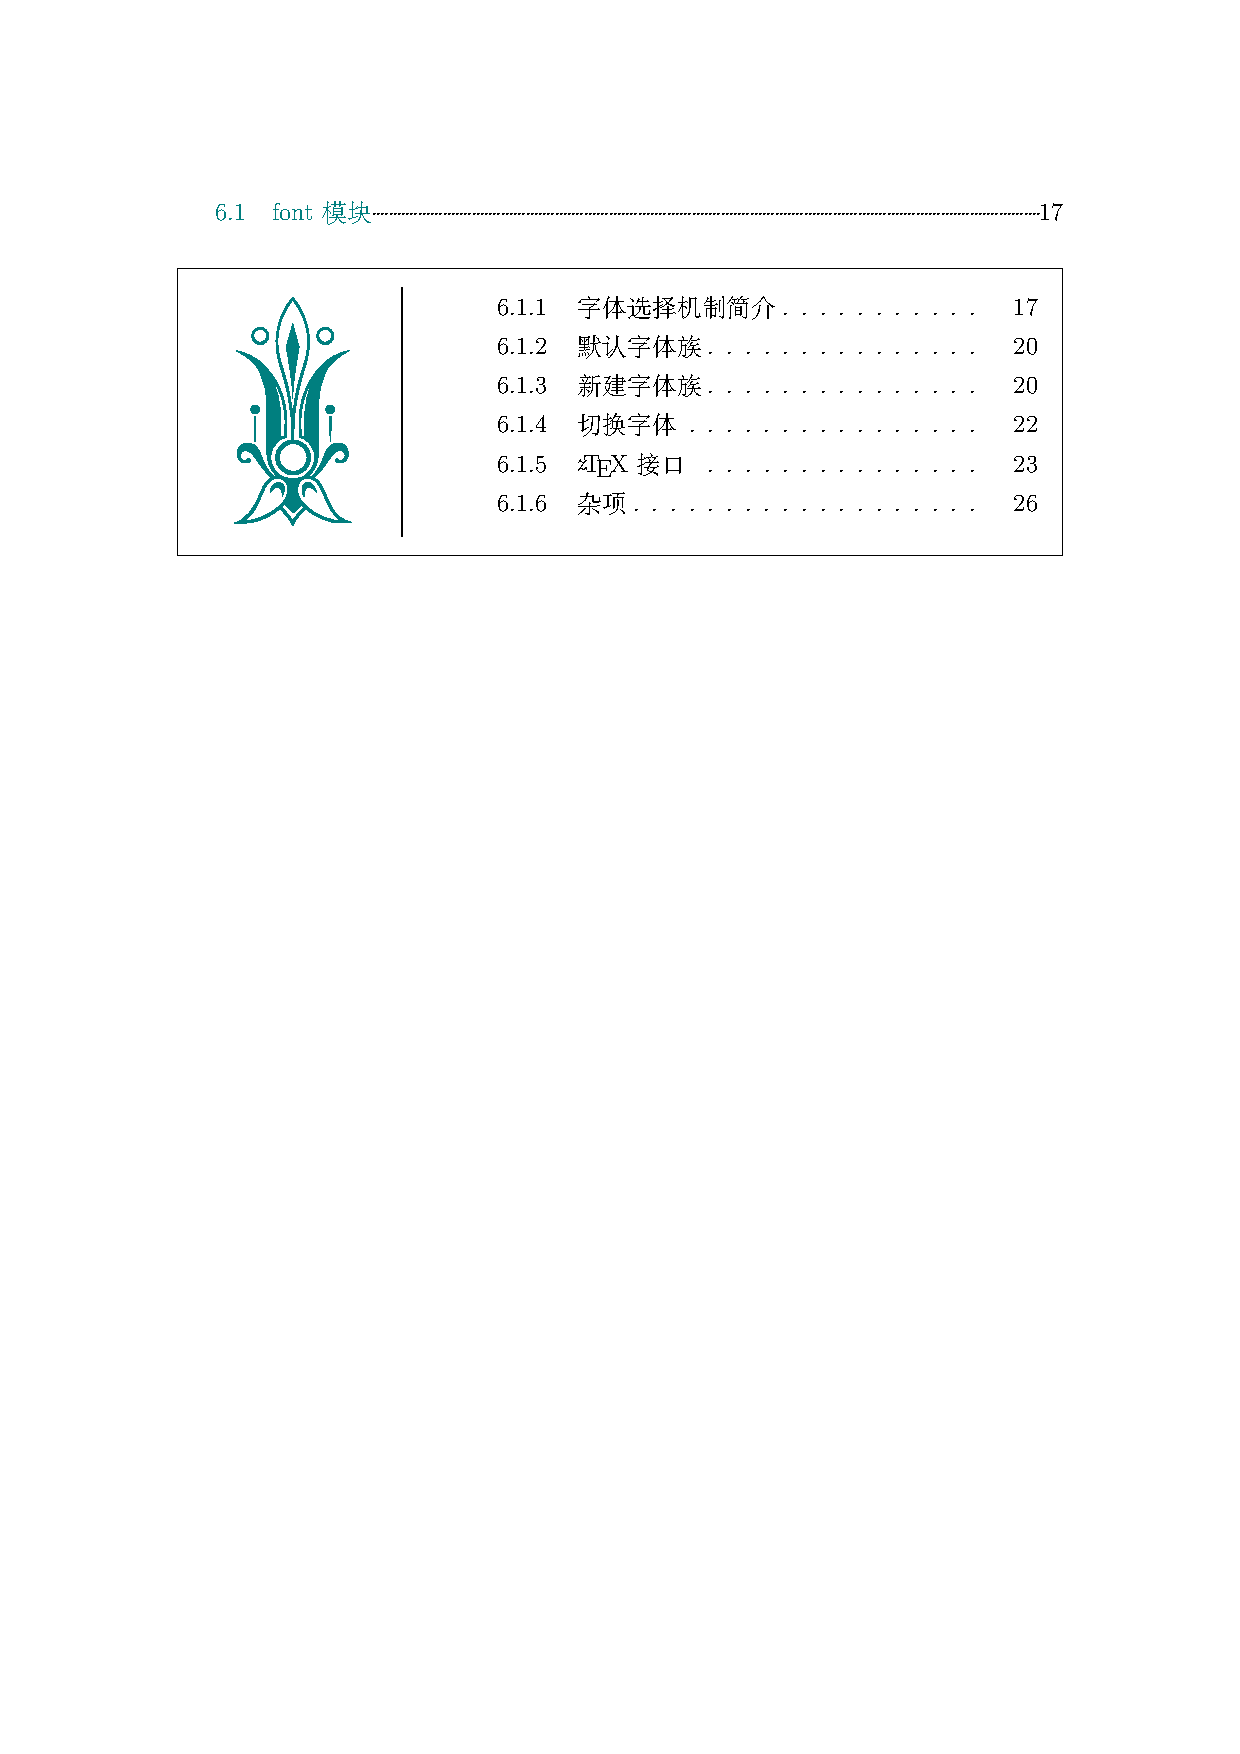
\includegraphics[width=\textwidth]{./support/pics/toc_group.pdf}

\paragraph{案例:2}\label{ztoc:hook-position} 下面这个案例清晰地展示了目录中这些 
hook 的位置关系, \fbox{BG:\meta{int}} 和 \fbox{EG:\meta{int}} 代表目录条目自身
局部组的开始和结束位置(这些局部组目前已被移除 -- 2025-09-12).
\vskip1.25em\relax
\begin{DocExample}*[++]
\ExplSyntaxOn
\int_new:N \g__test_toc_group_int
\AddToHook{ztoc/tocline/begin}
  {
    \fbox{BG:\int_use:N \g__test_toc_group_int}
  }
\AddToHook{ztoc/tocline/end}
  {
    \fbox{EG:\int_use:N \g__test_toc_group_int}
    \int_gincr:N \g__test_toc_group_int
  }
\cs_new:Npn \__debug_ztoc_hook:nn #1#2
  { \ztocgroupinsert{#1}{\fbox{\color{#2}\sffamily #1}} }

% begin/end hooks:
\__debug_ztoc_hook:nn {subsection,1,begin}{red}
\__debug_ztoc_hook:nn {subsection,1,end}{red}
\__debug_ztoc_hook:nn {subsubsection,5,begin}{gray}
\__debug_ztoc_hook:nn {subsubsection,5,end}{gray}
% new before/after hooks:
\__debug_ztoc_hook:nn {subsection,1,before}{blue}
\__debug_ztoc_hook:nn {subsection,1,after}{blue}
\__debug_ztoc_hook:nn {subsubsection,1,before}{teal}
\__debug_ztoc_hook:nn {subsubsection,1,after}{teal}
\__debug_ztoc_hook:nn {subsubsection,3,before}{purple}
\__debug_ztoc_hook:nn {subsubsection,3,after}{purple}
\ExplSyntaxOff
\zlocaltoc{subsection}{4}
\end{DocExample}
\RemoveFromHook{ztoc/tocline/begin}
\RemoveFromHook{ztoc/tocline/end}


\clearpage
\paragraph{案例:3} 这个案例相较之上一个案例更加复杂:

\begin{DocExample}*
\begingroup\makeatletter
\tocupdatelinewidthfix
\def\customtocthemecolor{teal}
\ztocformat\subsection
  {
    explicit=true,
    code={%
      \noindent\fcolorbox{white}{\customtocthemecolor}{\hb@xt@\linewidthfix
        {\bfseries\large\color{white}\ztocname
          \hskip.75em\relax\ztoctitle\hfill\ztocpage}}%
    }
  }
\ztocformat\subsubsection
  {
    format+=\color{\customtocthemecolor},
    page.format+=\color{\customtocthemecolor},
    name.before=\S\;
  }
\ztocgroupinsert{subsection,1,begin}%
  {%
    \begin{tcolorbox}[
      enhanced, sharp corners,
      boxrule=.5pt, colback=white,
      left=20pt, colframe=\customtocthemecolor,
      overlay={
        \ornamentcorner{north west}{north west}{0}
        \ornamentcorner{north west}{south west}{90}
        \ornamentcorner{north west}{south east}{180}
        \ornamentcorner{north west}{north east}{270}
      }
    ]
    \pgfornament[width = 2.5cm,color = \customtocthemecolor]{8}%
    \kern-6pt\relax\begin{minipage}{.75\linewidth}%
  }
\ztocgroupinsert{subsection,1,end}%
  {%
    \end{minipage}%
    \end{tcolorbox}%
  }
\zlocaltoc{subsection}{4}
\makeatother\endgroup
\end{DocExample}


\clearpage
\paragraph{案例:4} 我们可以使用 \cmd{\ztocgroupinsert} 命令复刻 \pkg{titletoc}
宏包所提供的样式:

\begin{DocExample}*
\makeatletter
\def\customssstyle#1{%
  \ztocgroupinsert{subsection,#1,begin}
    {\raggedright\hangindent2.3em\relax\noindent\hskip2.3em\relax【}
  \ztocgroupinsert{subsection,#1,end}{】\par}
}
\makeatother
\customssstyle{1} \customssstyle{2}
\customssstyle{3} \customssstyle{4}
{
  \ztocformat\subsubsection{
    explicit=true,
    code={%
      \textit{\ztocname\enskip\ztoctitle\enskip
      (\ztochyperpage{\ztocpage})\ztociflast{}{;}\enskip}}
  }
  \ztocformat\subsection{
    explicit=true,
    code = {%
      \S\;\ztocname\enskip\ztoctitle
      \hskip1em\ztochyperpage{\ztocpage}\par}
  }
  \begin{multicols}{2}
    \zlocaltoc{subsection}{4, 11, 8, 6}
  \end{multicols}
}
\end{DocExample}



\clearpage
\setcounter{tocdepth}{3}
\paragraph{案例: 5} 这个案例相较之上一个案例更加复杂:

\begin{DocExample}*
\begingroup\makeatletter
% \setcounter{tocdepth}{3}
\def\customtocthemecolor{SeaGreen}
\ztocformat\section
  {
    explicit=true,
    code={%
      \noindent\hskip1.5em\fcolorbox{white}{\customtocthemecolor}{\hb@xt@
        \dimexpr\linewidth-2\fboxsep-1.5em\relax
        {\bfseries\large\color{white}第\zhnumber{\ztocname}节
          \hskip.75em\relax\ztoctitle\hfill\ztocpage}}%
    }
  }
\ztocformat\subsection{
  name.before=\S\;, name.width=2.7em,
  format+=\color{\customtocthemecolor},
  page.format+=\color{\customtocthemecolor},
  leader.sep=2pt, page.width=1em,
  hyper.title=true,
  leader.content=\textcolor{\customtocthemecolor}{.},
}
\ztocgroupinsert{section,1,before}%
  {%
    \begin{tcolorbox}[
      enhanced, sharp corners,
      boxrule=.5pt, colback=white,
      left=20pt, colframe=\customtocthemecolor,
      overlay={
        \ornamentcorner{north west}{north west}{0}
        \ornamentcorner{north west}{south west}{90}
        \ornamentcorner{north west}{south east}{180}
        \ornamentcorner{north west}{north east}{270}
      }
    ]
    \pgfornament[width = 2.5cm,color = \customtocthemecolor]{10}%
    \begin{minipage}{.77\linewidth}%
  }
\ztocgroupinsert{section,1,begin}{%
  % \setlength{\columnsep}{0em}
  \begin{multicols}{2}}
\ztocgroupinsert{section,1,after}%
  {%
    \end{multicols}%
    \end{minipage}%
    \end{tcolorbox}%
  }
\zlocaltoc{section}{6}
\makeatother\endgroup
\end{DocExample}
\setcounter{tocdepth}{4}


\clearpage
\paragraph{案例: 6}\label{toc-longtable} 这个案例复刻了 \pkg{etoc} 中的目录样式(参见 \pkg{etoc} 宏包第 39 节):

\begin{dxample}[1]
\ztocgroupinsert{section,1,before}
  {\begin{longtable}{|l|l|r|}}
\ztocgroupinsert{section,4,after}
  {\\ \hline\end{longtable}}
{
  \ztocformat\section{
    explicit=true,
    code = {%
      \ztociffirst{\kill\hline\multicolumn{3}{|c|}{\large\bfseries Table of Contents}\\\hline}{\\\hline}%
      \multicolumn{3}{||c||}{\bfseries 第\;\ztocname\;节\enskip\ztoctitle}%
    }
  }
  \ztocformat\subsection{
    explicit=true,
    code ={\\\hline
      \textbf{\S\ztocname} & \ztocname\enskip\ztoctitle & \ztochyperpage{\ztocpage}
    }
  }
  \ztocformat\subsubsection{
    explicit=true,
    code = {\\
      & \ztocname\enskip\ztoctitle & \ztochyperpage{\ztocpage}
    }
  }
  \zlocaltoc{section}{1, 2, 7, 9}
}
\end{dxample}


\clearpage
\paragraph{案例: 7} 这个案例也是受到 \pkg{etoc} 宏包的启发 -- 将目录展示为思维导图的形式:

\begin{dxample}[1]
\definecolor{Green}{HTML}{15821b}
\tikzset{
  rootKey/.style={draw, rectangle, rounded corners, fill=Green, text=white},
}
\ExplSyntaxOn
\cs_new:Npn \__toc_tree:nn #1#2
  {
    \quark_if_no_value:nF {#1}
      {
        \Tree[.\node[rootKey]{#1};~#2 ]
      }
  }
\cs_generate_variant:Nn \__toc_tree:nn {oe}
\def\wraper#1{[.{\exp_not:n {#1}}~]}
\cs_new:Npn \ztoc_typeset_toctree:nnn #1#2#3
  {
    \ztoc_table_filter_key_byclass:nnnNN {#1}{#2}{#3}
      \g_ztoc_keyvaltoc_seq \g_tmpb_seq
    \seq_gpop_left:NN \g_tmpb_seq \secRoot
    \__toc_tree:oe { \secRoot }
      { \seq_map_function:NN \g_tmpb_seq \wraper }
  }
\def\TocTree#1#2#3
  {
    \exp_args:Nne \ztoc_typeset_toctree:nnn
      {#1}{#2}{#3}
  }
\ExplSyntaxOff

\noindent\begin{tikzpicture}[
    grow'=right,
    level distance=50pt,
    sibling distance=10pt,
    level 1/.style={level distance=25pt},
    every tree node/.style={anchor=west, draw, rectangle, rounded corners, fill=gray!25},
    every level 0 node/.style={anchor=east},
    edge from parent/.style={
      draw, thick, rounded corners,
      edge from parent path={
        (\tikzparentnode.east) -- +(10pt, 0pt)
        |- (\tikzchildnode.west)
      }
    },
  ]
  \TocTree{subsection}{4}{title}
  \begin{scope}[xshift=12cm]
    \TocTree{subsection}
      {\ztocindex{subsection}{\pkg{alias} 库}}
      {page}
  \end{scope}
\end{tikzpicture}
\end{dxample}


\clearpage
\paragraph{案例: 8} 这个案列相较之上一个案例更加复杂, 它展示了 \cmd{\ztoc_group_parser:NNNnnnnn} 命令
中 \meta{step code} 的使用方法:

\begin{dxample}[0]
% \usetikzlibrary { mindmap, trees }
\ExplSyntaxOn
\int_new:N \g__mindmap_color_int
\seq_new:N \g__mindmap_data_seq
\seq_new:N \g__mindmap_keyvaldata_seq
\tl_new:N \g__mindmap_filter_data_tl
\def\toclinecmd#1#2#3#4
  {
    % override hyperlink color.
    {\ztexlink{#1.#2}{\textcolor{white}{#3(#4)}}}
  }
\cs_new:Npn \__ztoc_gen_mindmap_data:nn #1#2
  {
    \tl_gclear:N \g_tmpa_tl
    \ztoc_table_filter_byclass:nnNN
      { #1 }{ #2 } 
      \g_ztoc_keyvaltoc_seq
      \g__mindmap_data_seq
    \ztoc_generate_keyvaltable_seq:NN
      \g__mindmap_data_seq
      \g__mindmap_keyvaldata_seq
    \ztoc_group_parser:NNNnnnnn \g__mindmap_keyvaldata_seq
      \toclinecmd \g_tmpa_tl
        {
          child [ concept~color = blue!
            \int_eval:n{\g__mindmap_color_int*6}!green
          ] \bgroup node[concept]
        }
      {}{}{\egroup}{\int_gincr:N \g__mindmap_color_int}
    % replace '\bgroup' and '\egroup' by '{' and '}'. 
    \str_clear:N \l_tmpa_str
    \exp_args:NNo \str_set:Nn \l_tmpa_str { \g_tmpa_tl }
    \exp_args:NNne \str_replace_all:Nnn \l_tmpa_str
      { \bgroup }{ \char_generate:nn {123}{12} }
    \exp_args:NNne \str_replace_all:Nnn \l_tmpa_str
      { \egroup }{ \char_generate:nn {125}{12} }
    \tl_gset_rescan:Nno \g__mindmap_filter_data_tl
      { \cctab_select:N \c_document_cctab }
      { \l_tmpa_str }
  }
\cs_new:Npn \__tkz_mind_map:n #1
  {
    \tl_if_empty:nF {#1}
      {
        \node[concept] 
          {\color{white}\ztex{}~Interface}
          #1;
      }
  }
\newcommand{\mindmap}[2]
  {
    \__ztoc_gen_mindmap_data:nn
      { #1 }{ #2 }
    \exp_args:No \__tkz_mind_map:n
      { \g__mindmap_filter_data_tl }
  }
\ExplSyntaxOff
\begin{tikzpicture}[
    mindmap, grow cyclic,
    text width=2cm, align=flush center,
    nodes={concept}, concept color=blue!60,
    root concept/.append style={
      text width=4cm, font=\Large
    },
    level 1 concept/.append style={
      font=\normalsize, color=white
    },
    level 1/.append style={
      level distance=5cm, sibling angle=45,
      text width=3cm, font=\Large
    },
    level 2/.append style={
      level distance=9cm, sibling angle=90,
      text width=3cm, font=\Large
    },
    level 3/.append style={
      level distance=5cm, sibling angle=45,
      text width=3cm, font=\Large
    },
  ]
  \mindmap{section}{7}
\end{tikzpicture}
\end{dxample}


% NOTE: 1. for that this figure is too big,
%          we compile it manually.
%       2. these commands have been declared
%          in the cover page.
\newgeometry{margin=0pt}
\thispagestyle{empty}
\mbox{}\vfill
\ExplSyntaxOn
% \int_new:N \g__mindmap_color_int
% \seq_new:N \g__mindmap_data_seq
% \seq_new:N \g__mindmap_keyvaldata_seq
\def\toclinecmd#1#2#3#4
  {
    % override hyperlink color.
    {\ztexlink{#1.#2}{\textcolor{white}{#3(#4)}}}
  }

% \cs_new:Npn \__ztoc_gen_mindmap_data:nn #1#2
%   {
%     \ztoc_table_filter_byclass:nnNN
%       { #1 }{ #2 } 
%       \g_ztoc_keyvaltoc_seq
%       \g__mindmap_data_seq
%     \ztoc_generate_keyvaltable_seq:NN
%       \g__mindmap_data_seq
%       \g__mindmap_keyvaldata_seq
%     \ztoc_group_parser:NNNnnnnn \g__mindmap_keyvaldata_seq
%       \toclinecmd \g_tmpa_tl
%         {
%           child [ concept~color = blue!
%             \int_eval:n{\g__mindmap_color_int*6}!green
%           ] \bgroup node[concept]
%         }
%       {}{}{\egroup}{\int_gincr:N \g__mindmap_color_int}
%     % replace '\bgroup' and '\egroup' by '{' and '}'. 
%     \exp_args:NNo \str_set:Nn \l_tmpa_str { \g_tmpa_tl }
%     \exp_args:NNne \str_replace_all:Nnn \l_tmpa_str
%       { \bgroup }{ \char_generate:nn {123}{12} }
%     \exp_args:NNne \str_replace_all:Nnn \l_tmpa_str
%       { \egroup }{ \char_generate:nn {125}{12} }
%     \tl_gset_rescan:Nno \g_tmpa_tl
%       { \cctab_select:N \c_document_cctab }
%       { \l_tmpa_str }
%   }
% \cs_new:Npn \__tkz_mind_map:n #1
%   {
%     \tl_if_empty:nF {#1}
%       {
%         \node[concept] 
%           {\color{white}\ztex{}~Interface}
%           #1;
%       }
%   }
\newcommand{\mindmapAFTER}[2]
  {
    % \__ztoc_gen_mindmap_data:nn
    %   { #1 }{ #2 }
    \exp_args:No \__tkz_mind_map:n
      { \g__mindmap_filter_data_tl }
  }
\ExplSyntaxOff
\noindent\begin{tikzpicture}[
    mindmap, grow cyclic,
    text width=2cm, align=flush center,
    nodes={concept}, concept color=blue!60,
    root concept/.append style={text width=4cm, font=\Large},
    level 1/.append style={level distance=5cm, sibling angle=45, text width=3cm, font=\Large},
    level 2/.append style={level distance=8.75cm, sibling angle=90, text width=3cm, font=\Large},
    level 3/.append style={level distance=5cm, sibling angle=45, text width=3cm, font=\Large},
    level 1 concept/.append style={font=\normalsize, color=white},
  ]
  \mindmapAFTER{section}{7}
\end{tikzpicture}
\vfill\mbox{}
\restoregeometry


% \clearpage
\newgeometry{left=2.5cm, right=2.5cm}
\paragraph{案例: 9} 下面这个案例展示了 \cmd{\ztociffirst}, \cmd{\ztociflast} 以及 \cmd{\ztocdepth}
等命令的使用方法:

\begin{dxample}[0]
\ExplSyntaxOn
\newcommand{\nbraket}
  { \makebox[0pt]{\rule[-7.5pt]{.75pt}{19pt}} }
\newcommand{\ubraket}
  {
    \makebox[0pt]{
      \rule[-7pt]{.75pt}{10pt}
    }
    \makebox[0pt][l]{
      \kern-.375pt\raise3pt\hbox{\rule{3pt}{.75pt}}
    }
  }
\newcommand{\bbraket}
  {
    \makebox[0pt]{ \rule[3pt]{.75pt}{10pt} }
    \makebox[0pt][l]
      { \kern-.375pt\raise3pt
      \hbox{\rule{3pt}{.75pt}} }
  }
\newcommand{\showbar}
  {
    \prg_replicate:nn {\ztocdepth - 2}
      { \kern20pt \nbraket }
    \kern20pt \ztociffirst { \ubraket }
      { \ztociflast{\bbraket}{\nbraket} }
  }
\ztocformat{\section, \subsection, \subsubsection}
  {
    explicit=true,
    code = {
      \noindent
      \prg_replicate:nn {\ztocdepth-1}
        {
          \hskip 20pt\relax
        }
      \llap{\smash{\showbar}}
      \kern10pt
      \ztoctitle\par
    }
  }
\ExplSyntaxOff
{
  \ztocformat\subsection{ignore.name={10.}}
  \ztocformat\subsubsection{ignore.name={10.}}
  \multicolcontents{2}
}
\end{dxample}

\newgeometry{margin=0pt}
\thispagestyle{empty}
\begin{center}
  \mbox{}\vfill
  \includegraphicsifexsit[height=.95\paperheight]{./support/pics/toclevel.pdf}
  \vfill\mbox{}
\end{center}
\restoregeometry


\newgeometry{left=2.5cm, right=2.5cm}
\paragraph{案例: 10} 下面这个案例相较之上一个案例更加复杂, 但它展示了 \cmd{\ztoc_group_parser:NNNnnnnn} 命令的
强大和普适性:

\begin{dxample}[0]
% \usepackage{tikz}
% \usepackage{tikz-qtree}
% \usepackage{tikz-qtree-patch}
\definecolor{Red}{HTML}{e32b2d}
\definecolor{Green}{HTML}{15821b}
\definecolor{Blue}{HTML}{0984e3}
\tikzset{
  section/.style={draw, rectangle, rounded corners, fill=Red},
  subsection/.style={draw, rectangle, rounded corners, fill=Blue, text=white},
  subsubsection/.style={draw, rectangle, rounded corners, fill=Green, text=white},
}
\ExplSyntaxOn
% \def\toclinecmd#1#2#3#4{{#1:#2:#3:#4}~}
\def\toclinecmd#1#2#3#4{{\gparserclass(\gparserindex):#2:#3:#4}~}
\ztoc_group_parser:NNNnnnnn \g_ztoc_keyvaltoc_seq
  \toclinecmd \g_tmpa_tl {[.}{}{}{~]}{}
\def\TocTree
  {
    \exp_args:Nno \__toc_tree:nn
      {\ztex{}~接口文档}
      {\g_tmpa_tl}
  }
\cs_new:Npn \__toc_tree:nn #1#2
  {
    \quark_if_no_value:nF {#1}
      {
        \Tree[.\node[section]{#1};~#2 ]
      }
  }
\ExplSyntaxOff

\thispagestyle{empty}
\begin{tikzpicture}[
    grow'=right, level distance=1cm,
    sibling distance=10pt,
    every tree node/.style = {
      anchor=west, outer sep=0pt, draw, rectangle, 
      rounded corners, fill=gray!25
    },
    every level 1 node/.style = {
      subsection
    },
    every level 2 node/.style = {
      subsubsection
    },
    edge from parent/.style={
      draw, thick, rounded corners,
      edge from parent path={
        (\tikzparentnode.east) -- +(.5cm, 0pt)
        |- (\tikzchildnode.west)
      },
    },
  ]
  \TocTree
\end{tikzpicture}
\end{dxample}


\newgeometry{margin=0pt}
\thispagestyle{empty}
\begin{center}
  \mbox{}\vfill
  \includegraphicsifexsit[height=.95\paperheight]
    {./support/pics/toctree.pdf}
  \vfill\mbox{}
\end{center}
\restoregeometry



\clearpage
\subsubsection{编程接口:初始化}\label{sect:toc_iow}
本小节描述的命令在章节命令或目录相关的制作过程中都是不可或缺的, 我们在这里对它们进行一个统一规范的描述.

\begin{function}[added=2025-09-03]{\c_zsect_level_leagcy_prop}
  该变量记录了原 \hologo{LaTeX2e} 中(常规)章节的层级信息, 此变量目前未被使用.
\end{function}


\begin{function}[added=2025-09-03]{
    \g_zsect_level_int,
    \c_zsect_level_prop,
    \c_zsect_level_clist,
    \c_zsect_level_tl,
  }
  这些变量记录了文档中的常规章节命令信息(不包括 ``\texttt{figure, table, ...} 等''), 在任何情况下, 
  用户都不应该修改它们. \cmd{\g_zsect_level_int} 表示当前文档中常规章节类型的数量; \cmd{\c_zsect_level_prop}
  记录了每一个常规章节类型对应的层级.
\end{function}


\begin{function}[added=2025-09-03]
  {
    \c_ztoc_special_level_prop, 
    \c_ztoc_special_level_clist,
  }
  这两个变量记录了文档中的非常规(章节)命令层级信息, 比如 \texttt{figure, table, ...} 等.
\end{function}


\begin{function}[added=2025-09-10]{\c_ztoc_table_types_clist, \c_ztoc_table_types_prop}
  这两个变量记录了非常规(章节)目录文件的后缀. \cmd{\c_ztoc_table_types_prop} 记录了从 ``\texttt{figure, table, ...}'' 到 
  目录文件后缀的映射, 其中 ``\texttt{toc}'' 对应的键(key)为 ``\texttt{sect}''. 
\end{function}


\begin{function}[added=2025-09-03]{\zsect_config_sync:nn}
  \begin{syntax}
    \cmd{\zsect_config_sync:nn} \Arg{class}\Arg{level}
  \end{syntax}
  此命令用于同步章节命令和目录相关的(初始化)变量.
\end{function}


\begin{function}[added=2025-09-03]{\zsect_class_level_remap:n}
  \begin{syntax}
    \cs{zsect_class_level_remap:n} \Arg{keyval}
  \end{syntax}
  此命令封装自上述的 \cmd{\zsect_config_sync:nn} 命令, 加入了错误处理, 同步了一些其余的变量.
  当用户需要自定义章节或目录类型时, 请使用此命令进行同步(除非你清楚相关原理, 否则不建议使用 
  \cmd{\zsect_config_sync:nn} 命令进行同步).\par\vskip.72em\relax
  \noindent{\color{red}\sffamily NOTE: 用户层面的 \cs{zseclevelmap} 基于此命令.}
\end{function}


\begin{function}[added=2025-09-03, EXP]{
    \ztoc_get_class_level_expandable:n,
    \ztoc_get_class_level_expandable:o,
    \ztoc_get_class_level_expandable:e,
  }
  \begin{syntax}
    \cs{ztoc_get_class_level_expandable:n} \Arg{class}
  \end{syntax}
  此命令会返回当前文档类中 \meta{class} 对应的层级, 为一个整数.
\end{function}


\begin{function}[added=2025-09-03]{
    \ztoc_get_class_level:Nn,
    \ztoc_get_class_level:No,
    \ztoc_get_class_level:Ne,
  }
  \begin{syntax}
    \cs{ztoc_get_class_level:Nn} \meta{macro} \Arg{class}
  \end{syntax}
  此命令会返回当前文档类中 \meta{class} 对应的层级, 为一个整数, 其
  被置于 \meta{macro} 这个宏中.
\end{function}


\begin{function}[added=2025-09-03]{
    \g_ztoc_toc_iow,
    \g_ztoc_lof_iow,
    \g_ztoc_lot_iow,
    \g_ztoc_log_iow,
    \g_ztoc_lom_iow,
    \g_ztoc_loa_iow,
    \g_ztoc_lol_iow,
  }
  \ztex{} 预先创建了这些 stream 接口用于目录文件的写入操作. 它们的含义如下: 
  \vspace*{-.8em}
  \begin{multicols}{2}
  \begin{itemize}
    \item \cs{g_ztoc_toc_iow}: (章节)目录;
    \item \cs{g_ztoc_lof_iow}: 图片目录;
    \item \cs{g_ztoc_lot_iow}: 表格目录;
    \item \cs{g_ztoc_log_iow}: 术语目录;
    \item \cs{g_ztoc_lom_iow}: 定理目录;
    \item \cs{g_ztoc_loa_iow}: 算法目录;
    \item \cs{g_ztoc_lol_iow}: 代码目录.
  \end{itemize}
  \end{multicols}
  \vskip-.8em\relax
  % \par\vskip1.5em\relax
  \noindent{\color{red}\sffamily NOTE: 除非你清楚相关原理，否则建议保持这些变量的默认设置.}
\end{function}


\begin{function}[added=2025-09-03]{
    \g_ztoc_toc_iow_bool,
    \g_ztoc_lof_iow_bool,
    \g_ztoc_lot_iow_bool,
    \g_ztoc_log_iow_bool,
    \g_ztoc_lom_iow_bool,
    \g_ztoc_loa_iow_bool,
    \g_ztoc_lol_iow_bool,
  }
  这些 bool 变量用于检测相应的目录写入接口是否可用, 该类型的目录启用后, 对应的 bool 
  变量值为 \texttt{true}.
  \par\vskip1.5em\relax\noindent{\color{red}\sffamily NOTE: 除非你清楚相关原理，否则建议保持这些变量的默认设置.}
\end{function}


\begin{function}[added=2025-09-03]{
    \g_ztoc_toc_seq,
    \g_ztoc_lof_seq,
    \g_ztoc_lot_seq,
    \g_ztoc_log_seq,
    \g_ztoc_lom_seq,
    \g_ztoc_loa_seq,
    \g_ztoc_lol_seq,
  }
  这些变量记录了全局目录数据, 用户层面的 \cmd{\tableofcontents}, \cmd{\multicolcontents} 命令
  均基于这里的 \cmd{\g_ztoc_toc_seq} 变量.
  \par\vskip1.5em\relax\noindent{\color{red}\sffamily NOTE: 除非你清楚相关原理，否则建议保持这些变量的默认设置.}
\end{function}


\begin{function}[added=2025-09-03]{
    \g_ztoc_keyvaltoc_seq,
    \g_ztoc_keyvallof_seq,
    \g_ztoc_keyvallot_seq,
    \g_ztoc_keyvallog_seq,
    \g_ztoc_keyvallom_seq,
    \g_ztoc_keyvalloa_seq,
    \g_ztoc_keyvallol_seq,
  }
  这些变量记录了对应的目录数据, 它们以键值的形式存储, 主要用于目录的筛选. 
  比如, \cmd{\ztoc_table_filter_byclass:nnNN} 命令, 其依赖于这里
  的 \cmd{\g_ztoc_keyvaltoc_seq} 变量.
  \par\vskip1.5em\relax\noindent{\color{red}\sffamily NOTE: 除非你清楚相关原理，否则建议保持这些变量的默认设置.}
\end{function}


\begin{function}[added=2025-09-03]{
    \g_ztoc_localtoc_seq,
    \g_ztoc_locallof_seq,
    \g_ztoc_locallot_seq,
    \g_ztoc_locallog_seq,
    \g_ztoc_locallom_seq, 
    \g_ztoc_localloa_seq,
    \g_ztoc_locallol_seq,
  }
  这些变量用于局部目录的排版. 比如, 用户层面的 \cs{zlocaltoc} 命令, 其筛选得到的目录数据
  保存于 \cmd{\g_ztoc_localtoc_seq} 这个变量中.
  \par\vskip1.5em\relax\noindent{\color{red}\sffamily NOTE: 除非你清楚相关原理，否则建议保持这些变量的默认设置.}
\end{function}


\clearpage
\subsubsection{编程接口:章节命令}
本小节描述的命令均与章节命令相关, 涉及到章节命令的创建, 样式自定义, 层级调整以及章节命令的
一些附属命令.

\paragraph{书签管理} 考虑到 tagged pdf 支持, 目前和 bookmark 相关的接口命令较少, 后续会有补充.
\begin{function}[added=2025-09-03]{
    \zsect_bookmark_add:nnn,
    \zsect_bookmark_add:ene,
    \zsect_bookmark_add:eee,
  }
  \begin{syntax}
    \cmd{\zsect_bookmark_add:nnn} \Arg{level}\Arg{content}\Arg{anchor}
  \end{syntax}
  此命令封装自 \pkg{hyperref} 宏包, 用于手动添加书签.
\end{function}


\paragraph{marks}
后续会出现 ``\texttt{class}'' 和 ``\texttt{mark class}'' 两个词, 这里做一个简短的说明:
前者表示章节命令 \texttt{class}, 可以叫做 ``\texttt{title class}''; 后者表示 mark 中的
class 名称.

\begin{function}[added=2025-09-03]{\zsect_mark_new_class_safe:nn}
  \begin{syntax}
    \cmd{\zsect_mark_new_class_safe:nn} \Arg{bool}\Arg{mark class}
  \end{syntax}
  此命令用于建立新的 mark class, 如果 \meta{mark class} 已存在, 则该命令会抛出错误;
  \meta{bool} 为 \cmd{\c_true_bool} 时会额外创建 ``\meta{mark class}-nonempty''
  这个 mark class.
\end{function}


\begin{function}[added=2025-09-03]{\zsect_right_mark_insert:n}
  \begin{syntax}
    \cmd{\zsect_right_mark_insert:n} \Arg{content}
  \end{syntax}
  此命令会将 \meta{content} 插入 ``\texttt{ztex-right}'' 和 ``\texttt{ztex-right-nonempty}''
  (如果 \meta{content} 非空) 这两个 mark class 中. 
\end{function}


\begin{function}[added=2025-09-03]{\zsect_mark_insert:nn}
  \begin{syntax}
    \cmd{\zsect_mark_insert:nn} \Arg{class}\Arg{content}
  \end{syntax}
  此命令用于更新 mark 列表(其会自动处理 \texttt{nonempty} mark class 中的内容), 和 \hologo{LaTeX2e} 中的 \cs{markright}, \cs{markboth} 作用类似.
  \meta{class} 表示标题的类型, 可选值有 \texttt{chapter, section, subsection, ...} 等; \meta{content}
  为自定的 mark 内容.\par\vskip0.73em\relax
  \noindent\textbf{注意}: 在 \cls{article} 中, \verb|\zsectmarkinsert{section}{content}| 的作用相当于原始的 
  \verb|\markboth{content}{}| 命令; 但是在 \cls{book} 文档类中, 其作用相当于 \verb|\markright{content}| 命令.
\end{function}


\begin{function}[added=2025-09-03]{
    \zsect_mark_user_insert:nn,
    \zsect_mark_user_insert:Vn,
    \zsect_mark_user_insert:ee,
  }
  \begin{syntax}
    \cmd{\zsect_mark_user_insert:nn} \Arg{class}\Arg{content}
  \end{syntax}
  此命令\textbf{只能}用于向\textbf{新}建立的 \meta{class} 中插入 \meta{content}, 不会影响原始的
  几个 mark class(其会自动处理 \texttt{nonempty} mark class 中的内容). 比如, 
  运行命令 \verb|\zsect_class_level_remap:n {book=0}| 后,
  \ztex{} 随即便创建了 ``\texttt{book}'' 这个 \meta{class} 对应的 mark class; 使用
  \verb|\zsect_mark_user_insert:nn {book}{XXX}| 命令即可向 ``book'' 对应的这个 mark class 
  中插入内容 ``\texttt{XXX}''.\vskip0.78em\relax
  \noindent{\color{red}\sffamily NOTE: 也可以使用上述的 \cmd{\zsect_mark_insert:nn} 命令向%
  新建立的 mark class 中插入内容. }
\end{function}


\begin{function}[added=2025-09-03]{
    \zsect_markclass_lower_empty:n,
    \zsect_markclass_lower_empty:V,
    \zsect_markclass_lower_empty:o,
    \zsect_markclass_lower_empty:e,
  }
  \begin{syntax}
    \cmd{\zsect_markclass_lower_empty:n} \Arg{class}
  \end{syntax}
  此命令会向其下(level 值比 \meta{class} 大的)的所有 mark class 中插入空内容. 
  因为 \ztex{} 目前维护了 4 个主要的 mark class, 所以它会忽略所有 level 层级大于 4 
  的 title class.
\end{function}


\begin{function}[added=2025-09-03]{
    \zsect_robust_left_mark:,
    \zsect_robust_right_mark:,
  }
  这两个命令相较之原始的 \cs{leftmark} 和 \cs{rightmark} 命令更加的实用和健壮.
\end{function}


\paragraph{章节命令} 考虑到 tagged pdf 支持, 目前和章节命令相关的接口命令较少, 后续会有补充.

\begin{function}[added=2025-09-08]{
    \zsect_once_title:nnnnn,
    \zsect_once_title:nonnn,
    \zsect_once_title:nennn,
    \zsect_once_title:ooooo,
    \zsect_once_title:eeeee,
  }
  \begin{syntax}
    \cmd{\zsect_once_title:nnnnn} \Arg{keyval}
    ~~~~\Arg{class}\Arg{bool}\Arg{toc-content}\Arg{sec-content}
  \end{syntax}
  此命令用于排版一次性的标题, 不会影响其它标题格式. \meta{keyval} 用于指定标题的属性,
  可用的键值列表请参见: \cref{sect:keyval}; \meta{class} 用于指定标题的类别, 可选值有
  ``\texttt{section, chapter, ...}'' 等(所有位于 \cs{c_zsect_level_clist} 中的 \meta{class} 均可); 
  \meta{bool} 用于指定该标题是否需要编号, 当其为 \cs{c_true_bool} 时, 不显示编号, 为 \cs{c_false_bool} 时
  显示编号; \meta{toc-content} 用于指定目录中的内容, 可以置为空, 此时目录中的该条目使用 \meta{sec-content}; 
  \meta{sec-content} 用于指定标题内容.
\end{function}


\begin{function}[added=2025-07-06]{
    \zsect_define_title:Nnn,
    \zsect_define_title:Non,
    \zsect_define_title:Nen,
    \zsect_define_title:cnn,
    \zsect_define_title:con,
    \zsect_define_title:cen,
  }
  \begin{syntax}
    \cmd{\zsect_define_title:Nnn} \meta{class} \Arg{style}\Arg{keyval}
  \end{syntax}
  此命令用于定义标题, 所有可用的键值列表参见节首说明: \cref{sect:intro}. \meta{class} 可以
  是 ``\verb|\part, \section, \subsection|'' 等. \meta{style} 用于指定新建立的章节命令所属的样式.
  \textbf{备注}: 如果该 \meta{class} 目录条目的 instance 不存在, 此时用户需要手动指定, 
  请参见 \cs{zsecdefine} 命令中的设置样例.
  % \par\vskip0.64em\relax
  % \noindent{\color{red}\sffamily NOTE: \meta{keyval} 中必须指明 ``\texttt{class}'' 键对应的值.}
\end{function}



\begin{function}[added=2025-09-07, updated=2025-09-10]{
    \zsect_caption_use:nnn,
    \zsect_caption_use:ooo,
    \zsect_caption_use:eee,
  }
  \begin{syntax}
    \cmd{\zsect_caption_use:nnn} \Arg{class}\Arg{format}\Arg{content}
  \end{syntax}
  此命令用于手动添加 caption, 它会主动调用 \cs{zsect_add_\meta{class}_line:eeee} 命令添加目录. 
  \meta{class} 可选值有 ``\texttt{figure, table, theorem, lstlisting, algorithm, glossary}'';
  \meta{format} 用于指定 caption 的格式, 使用 \verb|#1| 表示其前缀, 使用 \verb|#2| 表示 caption 的内容;
  \meta{content} 为 caption 的内容, \ztex{} 会自动为其增加前缀: \cs{fnum@\meta{class}}. (当 \meta{content} 
  为空时, 中间的冒号 -- ``\texttt{:}'' 不会显示). \textbf{备注}: \meta{content} 中的脆弱命令可以不用保护.
\end{function}



\clearpage
\subsubsection{编程接口:目录}
本小节描述目录相关的编程接口, 它们与目录的: 启用, 更新以及格式化相关.
基于这些命令, 用户可以更加方便地去控制目录的生成与排版.
\vskip1.54em\relax
\noindent{\color{red}\sffamily NOTE: \pkg{sect} 模块重定义了原始的 \cmd{\numberline} 和 \cmd{\contentsline} 命令. }


\begin{function}[added=2025-09-03]{
    \ztoc_enable_table:nn, 
    \ztoc_enable_table_swap:nn
  }
  \begin{syntax}
    \cs{ztoc_enable_table:nn} \Arg{file}\Arg{table}
    \cs{ztoc_enable_table_swap:nn} \Arg{table}\Arg{file}
  \end{syntax}
  此二命令用于控制启用的目录类型, 只有当 \meta{table} 类型的目录启用后, 用户才能在后文中使用 \meta{table} 
  类型的目录; \meta{file}(\textbf{不能} 添加文件后缀) 和 \meta{table} 的格式和含义与 \cmd{\ztoc_generate_table_seq:nn} 一致.
  \par\vskip.75em\relax\noindent{%
    \color{red}\sffamily NOTE: 此命令基于前述的 \cmd{\ztoc_generate_table_seq:nn} 命令. }
\end{function}


\begin{function}[added=2025-09-03]{\ztoc_stop_table:n}
  \begin{syntax}
    \cmd{\ztoc_stop_table:n} \Arg{table}
  \end{syntax}
  此命令会停止目录的收集, 它之后的所有目录数据均不会被记录, 用户应慎用此命令.
  \meta{table} 可选值有 ``\texttt{toc, lof, lot}'' 等.
\end{function}


\begin{function}[added=2025-09-06]{\@dottedtocline}
  \begin{syntax}
    \cmd{\@dottedtocline} 
    ~~\Arg{level}\Arg{indent}\Arg{name width}\Arg{title}\Arg{page}
  \end{syntax}
  此命令和 \hologo{LaTeX2e} 中的 \cmd{\@dottedtocline} 定义和作用完全一致.
  \textbf{备注}: 更推荐用户使用后续的 \cmd{\dottedtocline:nnnnn} 命令.
\end{function}


\begin{function}[added=2025-09-03]{\dottedtocline:nnnnn}
  \begin{syntax}
    \cmd{\dottedtocline:nnnnn} 
    ~~\Arg{level}\Arg{indent}\Arg{name width}\Arg{title}\Arg{page}
  \end{syntax}
  此命令基于后续的 \cmd{\zdottedtocline:nnnnnnnnn} 命令, 用于输出目录条目.
  如果 \meta{title} 中含有 \cmd{\numberline} 命令, 此时 \meta{name width} 用于调整 
  \meta{name} 的宽度; 如果没有, 那么 \meta{name width} 会变为当前条目的第2行到最后一行
  的 \verb|\leftskip| 值.\par
  \noindent \textbf{注意}: 在 \hologo{LaTeX2e} 的原始 \cmd{\dottedtocline} 命令中,
  \meta{name width} 被称为 ``\texttt{num width}''. 
  \vskip.74em\relax
  \noindent{\color{red}\sffamily NOTE: 该命令之后可能会使用 \pkg{l3galley} 进行重写.}
\end{function}


\begin{function}[added=2025-09-03]{\zdottedtocline:nnnnnnnnn}
  \begin{syntax}
    \cmd{\zdottedtocline:nnnnnnnnn}
    ~~\Arg{level}\Arg{indent}\Arg{tocrmarg}
    ~~\Arg{name width}\Arg{title}\Arg{leader}
    ~~\Arg{page spec}\Arg{endline}\Arg{before skip}
  \end{syntax}
  相较于上述的 \cmd{\dottedtocline:nnnnn} 命令, 此命令更加灵活.
  \meta{page spec} 用于指定 leader 后的内容; \meta{endline} 会插入到行尾, 
  可以用于控制目录条目是否换行; \meta{before skip} 用于设置目录前的垂直间距.
  \par\noindent \textbf{注意}: 在 \hologo{LaTeX2e} 的原始 \cmd{\dottedtocline} 命令中,
  \meta{name width} 被称为 ``\texttt{num width}''. 
  \vskip.74em\relax
  \noindent{\color{red}\sffamily NOTE: 该命令之后可能会使用 \pkg{l3galley} 进行重写.}
\end{function}


\newgeometry{left=3cm, right=3cm}
下面这个案例展示了 \cmd{\dottedtocline:nnnnn} 和 \cmd{\zdottedtocline:nnnnnnnnn} 两个命令的使用方法:
\vskip1.25em\relax
\begin{DocExample}*
% \usepackage{lipsum}
\ExplSyntaxOn\makeatletter
\let\TTTa\dottedtocline:nnnnn
\let\TTTb\zdottedtocline:nnnnnnnnn
\def\ltxtocleader{
  \leaders\hbox
    {$ \m@th
      \mkern \@dotsep mu
      \hbox{.}
      \mkern \@dotsep mu
    $}\hfill
}
\def\tocsepline{\par\noindent\dotfill\par}
\makeatother\ExplSyntaxOff
\tocsepline
\TTTa{2}{2em}{8em}{Test Title \fbox{A}}{99}
\TTTa{2}{2em}{6em}{\lipsum[1][1-3]}{100}
\TTTa{2}{2em}{4em}{\numberline{1.1.3}\lipsum[1][1-3]}{111}

\tocsepline
\TTTb{2}{2em}{3em}{6em}{\lipsum[1][1-3]}{\ltxtocleader}
  {100}{\par}{2em plus 10pt}
\TTTb{2}{2em}{6em}{6em}{\numberline{1.1.3}\lipsum[1][1-3]}{\ltxtocleader}
  {\fcolorbox{blue}{gray}{111}}{\par}{2em plus 10pt}
\tocsepline
\end{DocExample}
\restoregeometry


\begin{function}[added=2025-09-08]{
    \ztoc_once_tocline:nnnn,
    \ztoc_once_tocline:nooo,
    \ztoc_once_tocline:neee,
    \ztoc_once_tocline:oooo,
    \ztoc_once_tocline:eeee,
  }
  \begin{syntax}
    \cmd{\ztoc_once_tocline:nnnn} \Arg{keyval}
    ~~~~\Arg{toc depth}\{\Arg{name}\Arg{title}\}\Arg{page}
  \end{syntax}
  此命令用于排版一次性的目录, 不会影响其它目录条目. \meta{keyval} 的可用键值列表请参见: \cref{ss2:toc};
  \meta{toc depth} 用于指定该条目所处的目录层级; \meta{name}, \meta{title}
  和 \meta{page} 的含义在之前已经做过说明, 这里不在复述.\par\vskip1.5em\relax
  \noindent{\sffamily\color{red}NOTE: 此命令不能直接使用, 其依赖于 \cmd{\ztoc@current@class} 这个变量; 用户
  需首先将 \cmd{\ztoc@current@class} 定义为 ``\texttt{section, figure, ...}'' 等 \meta{class} 后, 才能正常使用此命令.}
\end{function}


\begin{function}[added=2025-09-03]{
    \zsect_add_toc_line:nnnn,
    \zsect_add_toc_line:oooo,
    \zsect_add_toc_line:nnee,
    \zsect_add_toc_line:nnoe,
    \zsect_add_toc_line:eeoe,
    \zsect_add_toc_line:eeee,
  }
  \begin{syntax}
    \cmd{\zsect_add_toc_line:nnnn} 
    ~~~~\Arg{class}\{\{\meta{name}\}\{\meta{title}\}\} 
    ~~~~\Arg{page}\Arg{anchor}
  \end{syntax}
  该命令用于向文件 \verb|\jobname.toc| 中添加一条目录条目, 如果 toc 没有启用, 则该命令不会进行任何操作;
  上述各个参数的含义请参见 \cref{sect:intro}, 这里不再复述.
\end{function}


\begin{function}[added=2025-09-03]{
    \zsect_add_table_line:nnnn,
    \zsect_add_table_line:oooo,
    \zsect_add_table_line:eeee,
  }
  \begin{syntax}
    \cmd{\zsect_add_table_line:nnnn} 
    ~~~~\Arg{class}\{\{\meta{name}\}\{\meta{title}\}\} 
    ~~~~\Arg{page}\Arg{anchor}
  \end{syntax}
  此命令与 \cmd{\zsect_add_toc_line:nnnn} 命令类似, 但写入的目录文件为:
  \verb|\jobname.lot|.
\end{function}


\begin{function}[added=2025-09-03]{
    \zsect_add_figure_line:nnnn,
    \zsect_add_figure_line:oooo,
    \zsect_add_figure_line:eeee,
  }
  \begin{syntax}
    \cmd{\zsect_add_figure_line:nnnn}
    ~~~~\Arg{class}\{\{\meta{name}\}\{\meta{title}\}\} 
    ~~~~\Arg{page}\Arg{anchor}
  \end{syntax}
  此命令与 \cmd{\zsect_add_toc_line:nnnn} 命令类似, 但写入的目录文件为:
  \verb|\jobname.lof|.
\end{function}


\begin{function}[added=2025-09-06]{
    \zsect_add_theorem_line:nnnn,
    \zsect_add_theorem_line:oooo,
    \zsect_add_theorem_line:eeee,
  }
  \begin{syntax}
    \cmd{\zsect_add_theorem_line:nnnn}
    ~~~~\Arg{class}\{\{\meta{name}\}\{\meta{title}\}\} 
    ~~~~\Arg{page}\Arg{anchor}
  \end{syntax}
  此命令与 \cmd{\zsect_add_toc_line:nnnn} 命令类似, 但写入的目录文件为:
  \verb|\jobname.lot|.
\end{function}


\begin{function}[added=2025-09-06]{
    \zsect_add_lstlisting_line:nnnn,
    \zsect_add_lstlisting_line:oooo,
    \zsect_add_lstlisting_line:eeee,
  }
  \begin{syntax}
    \cmd{\zsect_add_lstlisting_line:nnnn}
    ~~~~\Arg{class}\{\{\meta{name}\}\{\meta{title}\}\} 
    ~~~~\Arg{page}\Arg{anchor}
  \end{syntax}
  此命令与 \cmd{\zsect_add_toc_line:nnnn} 命令类似, 但写入的目录文件为:
  \verb|\jobname.lol|.
\end{function}


\begin{function}[added=2025-09-06]{
    \zsect_add_glossary_line:nnnn,
    \zsect_add_glossary_line:oooo,
    \zsect_add_glossary_line:eeee,
  }
  \begin{syntax}
    \cmd{\zsect_add_glossary_line:nnnn}
    ~~~~\Arg{class}\{\{\meta{name}\}\{\meta{title}\}\} 
    ~~~~\Arg{page}\Arg{anchor}
  \end{syntax}
  此命令与 \cmd{\zsect_add_toc_line:nnnn} 命令类似, 但写入的目录文件为: \verb|\jobname.log|.
  \vskip1.25em\relax
  \noindent{\sffamily\color{red}NOTE: 此命令现在还未完全适配, 用户暂时不要使用. }
\end{function}


\begin{function}[added=2025-09-06]{
    \zsect_add_algorithm_line:nnnn,
    \zsect_add_algorithm_line:oooo,
    \zsect_add_algorithm_line:eeee,
  }
  \begin{syntax}
    \cmd{\zsect_add_algorithm_line:nnnn} 
    ~~~~\Arg{class}\{\{\meta{name}\}\{\meta{title}\}\} 
    ~~~~\Arg{page}\Arg{anchor}
  \end{syntax}
  此命令与 \cmd{\zsect_add_toc_line:nnnn} 命令类似, 但写入的目录文件为:
  \verb|\jobname.loa|.
\end{function}


\begin{function}[added=2025-09-03]{
    \zsect_add_to_table:nn,
    \zsect_add_to_table:no,
    \zsect_add_to_table:oo,
    \zsect_add_to_table:ne,
    \zsect_add_to_table:ee,
  }
  \begin{syntax}
    \cmd{\zsect_add_to_table:nn} \Arg{table}\Arg{content}
  \end{syntax}
  此命令和上述的 \cmd{\zsect_add_toc_line:nnnn} 命令类似, 如果类型为 \meta{table} 的目录没有
  启用, 则该命令不会进行任何操作; \meta{content} 为写入的内容, 形式通常为:
  \vskip.15em\relax
    \verb|\contentsline{class}{{name}{title}}{page}{anchor}|
  \vskip.24em\relax
  \noindent\meta{table} 为 \meta{table} 类型, 可选值有 ``\texttt{toc, lot, lof, ...}'' 
  等.
\end{function}



\begin{function}[added=2025-09-03]{
    \ztoc_lcmd_setup:nn,  
    \ztoc_lcmd_setup:oo,  
    \ztoc_lcmd_setup:ee,
  }
  \begin{syntax}
    \cmd{\ztoc_lcmd_setup:nn} \Arg{class}\Arg{level}
  \end{syntax}
  此命令用于创建目录中相应的 \texttt{\char92l@\meta{class}} 命令,
  应用于 \texttt{chapter, section} 这样的常规 \texttt{class}; \meta{class} 
  中不包含 ``\verb|\|'', \meta{level} 为一个整数.
\end{function}


\begin{function}[added=2025-09-03]{ 
    \ztoc_special_lcmd_setup:nn,
    \ztoc_special_lcmd_setup:oo,
    \ztoc_special_lcmd_setup:ee,
  }
  \begin{syntax}
    \cmd{\ztoc_special_lcmd_setup:nn} \Arg{class}\Arg{level}
  \end{syntax}
  此命令用于创建目录中相应的 \texttt{\char92l@\meta{class}} 命令, 
  应用于 \texttt{figure, table} 这样的\textbf{非}常规 \texttt{class};
  \meta{class} 中不包含 ``\verb|\|'', \meta{level} 为一个整数.
\end{function}



\begin{function}[added=2025-09-03]{\ztoc_generate_table_seq:nn}
  \begin{syntax}
    \cs{ztoc_generate_table_seq:nn} \Arg{file}\Arg{table}
  \end{syntax}
  此命令用于生成目录对应的 seq 数据(变量 \cs{g_ztoc_\meta{table}_seq} 和变量 \cs{g_ztoc_keyval\meta{table}_seq}). 
  \meta{file} 为文件名, \textbf{不能} 包含文件的拓展名; \meta{table} 为目录类型, 所有可选值为: 
  ``toc, lot, lof, lom, loa, log, lol'', 分别代表 ``(章节)目录, 表格目录, 图片目录, 定理目录, 
  算法目录, 术语目录, 代码目录''.
\end{function}



\begin{function}[added=2025-09-19]{
    \ztoc_generate_keyvaltable_seq:NN,
    \ztoc_generate_keyvaltable_seq:cc,
  }
  \begin{syntax}
  \cs{ztoc_generate_keyvaltable_seq:NN} \meta{ori seq} \meta{seq}
  \end{syntax}
  此命令用于从 \meta{ori seq} 生成 keyval seq 变量 \meta{seq} (即, 变量 \cs{g_ztoc_keyval\meta{table}_seq}),
  且其赋值是全局的. \meta{ori seq} 可以使用后续的目录筛选命令生成, 如: \cmd{\ztoc_table_filter_byclass:nnNN};
  也可以使用 \pkg{ztool} 提供的 \cmd{\ztool_read_file_as_seq:nnN} 命令生成.
\end{function}



\begin{function}[added=2025-09-03]{
    \ztoc_generate_keyvaltable_seq:nN,
    \ztoc_generate_keyvaltable_seq:nc,
    \ztoc_generate_keyvaltable_seq:oN,
    \ztoc_generate_keyvaltable_seq:eN,
  }
  \begin{syntax}
    \cs{ztoc_generate_keyvaltable_seq:nN} \Arg{file} \meta{seq}
  \end{syntax}
  此命令用于从 \meta{file} 生成 keyval seq 数据(变量 \cs{g_ztoc_keyval\meta{table}_seq}), 且其赋值是全局的; 
  \meta{file} 中 \textbf{必须} 包含文件拓展名, 该文件中保存的目录类型可以是: ``(章节)目录, 表格目录, 
  图片目录, 定理目录, 算法目录, 术语目录''; 生成 keyval(seq) 数据保存于 \meta{seq} 变量中.  
  \par\vskip.75em\relax\noindent{\color{red}\sffamily NOTE: 前述的 \cmd{\ztoc_generate_table_seq:nn} 命令便是基于此命令和
  \pkg{ztool} 宏包中的 \cs{ztool_gread_file_as_seq:nnN} 命令}
\end{function}


\begin{function}[added=2025-09-12]{
    \ztoc_table_filter_key_byclass:nnnNN,
    \ztoc_table_filter_key_byclass:oooNN,
    \ztoc_table_filter_key_byclass:eeeNN,
    \ztoc_table_filter_key_byclass:nnncc,
    \ztoc_table_filter_key_byclass:eeecc,
  }
  \begin{syntax}
    \cmd{\ztoc_table_filter_key_byclass:nnnNN}
    ~~~~\Arg{class}\Arg{index}\Arg{key}
    ~~~~\meta{seq} \meta{filter seq}
  \end{syntax}
  此命令会从 \meta{seq} 变量中筛选目录条目, 并将筛选结果保存在 \meta{filter seq} 中(该赋值是全局的). 筛选规则
  由 \meta{class} 和 \meta{index} 指定: 筛选目录条目 \meta{key} 字段的值(筛选该条目及其包含的所有子目录); 
  \meta{class} 的可选值有 ``\texttt{chapter, section, ...}'' 等; \meta{index} 为一个整数, 表示所有 \meta{class} 
  条目的中该条目的绝对次序(更加详细的介绍可以参见 \cs{zlocaltoc} 命令); \meta{key} 的可选值
  有: ``\texttt{class, name, title, page, anchor, raw}''.
\end{function}


\begin{function}[added=2025-09-03, updated=2025-09-12]{
    \ztoc_table_filter_byclass:nnNN,
    \ztoc_table_filter_byclass:nncc,
    \ztoc_table_filter_byclass:neNN,
    \ztoc_table_filter_byclass:enNN,
    \ztoc_table_filter_byclass:eeNN,
    \ztoc_table_filter_byclass:eecc,
  }
  \begin{syntax}
  \cs{ztoc_table_filter_byclass:nnNN} 
  ~~~~\Arg{class}\Arg{index}
  ~~~~\meta{seq} \meta{filter seq}
  \end{syntax}
  此命令基于上述的 \cmd{\ztoc_table_filter_key_byclass:nnnNN} 命令, 用于从 \meta{seq} 变量中筛选目录条目, 
  并将筛选结果保存在 \meta{filter seq} 中(该赋值是全局的). 筛选规则由 \meta{class} 和 \meta{index} 指定: 
  筛选的是 ``\texttt{raw}'' 字段对应的值; \meta{class} 的可选值有 ``\texttt{chapter, section, ...}'' 等; 
  \meta{index} 为一个整数, 表示所有 \meta{class} 条目的中该条目的绝对次序(更加详细的介绍可以参见 \cs{zlocaltoc} 命令).
\end{function}


\begin{function}[added=2025-09-12]{
    \ztoc_table_filter_bynametitle:nnNN,
    \ztoc_table_filter_bynametitle:eeNN,
    \ztoc_table_filter_bynametitle:nncc,
    \ztoc_table_filter_bynametitle:eecc,
  }
  \begin{syntax}
  \cmd{\ztoc_table_filter_bynametitle:nnNN}
  ~~~~\Arg{name}\Arg{title}
  ~~~~\meta{seq}\meta{filter prop}
  \end{syntax}
  此命令会从 \meta{seq} 变量中筛选目录条目, 并将筛选结果保存在 \meta{filter prop} 中(该赋值是全局的).
  \meta{name} 和 \meta{title} 同时匹配的条目才会被筛选; \meta{filter prop} 表示筛选结果
  对应的键值(prop)变量, 如果不存在则返回空的键值变量; \meta{filter prop} 提供的键值可以
  参见: \cref{ztoc-example-data} 中 \texttt{data.ptoc} 文件.
  \vskip1.25em\relax
  \noindent{\sffamily\color{red}NOTE: \meta{name} 和 \meta{title} 比较的是字符串本身, 而不是 token 的比较;
  所以部分情况下, 用户需要将它们二者提前展开.}
\end{function}



\begin{function}[added=2025-09-15, rEXP]{
    \ztoc_tocline_index_byclasstitle:nnnN,
    \ztoc_tocline_index_byclasstitle:nnnc,
    \ztoc_tocline_index_byclasstitle:eeeN,
    \ztoc_tocline_index_byclasstitle:eeec,
  }
  \begin{syntax}
    \cmd{\ztoc_tocline_index_byclasstitle:nnnN}
    ~~~~\Arg{class}\Arg{title}
    ~~~~\Arg{bool}\meta{seq}
  \end{syntax}
  此命令用于确定目录条目在 \meta{seq} 变量中索引, 并且在 \texttt{e}-type 中可以被完全展开.
  目录条目由 \meta{class} 和 \meta{title} 确定, 二者需要同时匹配; 如果 \meta{seq} 中没有匹配的条目, 
  此命令总是返回一个小于零的整数值; 当 \meta{bool} 为 \cmd{\c_true_bool} 时, 此命令返回\textbf{相对}索引,
  即该条目在所有相同 \meta{class} 目录条目中的索引; 当 \meta{bool} 为 \cmd{\c_false_bool} 时,
  此命令返回\textbf{绝对}索引, 即该条目在整个目录中的所用, 不考虑 \meta{class}. 
\end{function}



\begin{function}[added=2025-09-12, rEXP]{
    \ztoc_tocline_index_bynametitle:nnN,
    \ztoc_tocline_index_bynametitle:nnc,
    \ztoc_tocline_index_bynametitle:eeN,
    \ztoc_tocline_index_bynametitle:eec,
  }
  \begin{syntax}
    \cmd{\ztoc_tocline_index_bynametitle:nnN}
    ~~~~\Arg{name}\Arg{title} \meta{seq}
  \end{syntax}
  此命令用于确定目录条目在 \meta{seq} 变量中\textbf{绝对}索引, 并且在 \texttt{e}-type 中可以被完全展开.
  目录条目由 \meta{name} 和 \meta{title} 确定, 二者需要同时匹配; 如果\meta{seq} 中没有匹配的条目, 
  此命令总是返回一个小于零的整数值. \textbf{备注}: 此命令无法返回\textbf{相对}索引.
  \vskip1.25em\relax
  \noindent{\sffamily\color{red}NOTE: \meta{name} 和 \meta{title} 比较的是字符串本身, 而不是 token 的比较;
  所以部分情况下, 用户需要将它们二者提前展开.}
\end{function}


\begin{function}[added=2025-09-15, rEXP]{\ztoc_tocline_level_bynametitle:Nnnn}
  \begin{syntax}
  \cmd{\ztoc_tocline_level_bynametitle:Nnnn}
  ~~~~\meta{seq}\Arg{name}\Arg{title}\Arg{offset}
  \end{syntax}
  此命令首先通过 \meta{name} 和 \meta{title} 确定初始目录条目的索引; 当确定此条目后,
  可以通过偏移值(此为一个整数) \meta{offset} 指定一条(新)目录条目, 返回(新)指定条目的 class level.
  \textbf{备注}: 此命令基于上述的 \cmd{\ztoc_tocline_index_bynametitle:nnN} 命令.
\end{function}



\begin{function}[added=2025-09-15, pTF, rEXP]{
    \ztoc_tocline_level_compare:Nnnnnn,
    \ztoc_tocline_level_compare:cnnnnn,
    \ztoc_tocline_level_compare:Neennn,
    \ztoc_tocline_level_compare:ceennn,
  }
  \begin{syntax}
    \cmd{\ztoc_tocline_level_compare:NnnnnnTF}
    ~~~~\meta{seq}\Arg{name}\Arg{title}
    ~~~~\Arg{offset_1}\Arg{offset_2}\Arg{relation}
    ~~~~\Arg{true code}\Arg{false code}
  \end{syntax}
  此命令首先通过 \meta{name} 和 \meta{title} 确定目标目录在 \meta{seq} 中的索引,
  在此基础上, \meta{offset_1} 和 \meta{offset_2} 指定了其余的两条目录条目;
  随后比较这两条目录条目的 class level, 比较方法由 \meta{relation} 指定, 可以选择:
  ``\verb|<, =, <, <=, >=|'' 等. \textbf{备注}: 此命令基于上述的 
  \cmd{\ztoc_tocline_index_bynametitle:nnN} 命令; 此命令在 \texttt{f}-型参数中\textbf{无法}被
  完全展开.
\end{function}



\begin{function}[added=2025-09-18, rEXP]{
    \ztoc_tocline_card:nnN,
    \ztoc_tocline_card:ooN,
    \ztoc_tocline_card:eeN,
    \ztoc_tocline_card:nnc,
    \ztoc_tocline_card:eec,
  }
  \begin{syntax}
  \cmd{\ztoc_tocline_card:nnN} 
  ~~~~\Arg{class}\Arg{title} \meta{seq}
  \end{syntax}
  此命令返回由 \meta{class} 和 \meta{title} 所确定目录的\textbf{子}目录(card 即 cardinality),
  如果由 \meta{class} 和 \meta{title} 所确定目标目录不存在, 其返回 ``-1''; \meta{seq} 为目录对应
  的 keyval seq 变量, 即 \texttt{\char92g_ztoc_keyval\meta{table}_seq}.
\end{function}



\begin{function}[added=2025-09-18, rEXP]{
    \ztoc_tocline_level_data:N,
    \ztoc_tocline_hilevel:N,
    \ztoc_tocline_lolevel:N,
    \ztoc_tocline_level_data:c,
    \ztoc_tocline_hilevel:c,
    \ztoc_tocline_lolevel:c,
  }
  \begin{syntax}
    \cmd{\ztoc_tocline_level_data:N} \meta{seq}
    \cmd{\ztoc_tocline_hilevel:N} \meta{seq}
    \cmd{\ztoc_tocline_lolevel:N} \meta{seq}
  \end{syntax}
  这系列的命令返回 \meta{seq} 中的 class level 数据, \meta{seq} 为目录对应
  的 keyval seq 变量. \cmd{\ztoc_tocline_level_data:N} 会返回所有目录条目
  的 level 值; 而 \cmd{\ztoc_tocline_hilevel:N} 或 \cmd{\ztoc_tocline_lolevel:N}
  只返回 \meta{seq} 中最小的 level 值或最大的 level 值(因为 \meta{class} 级别越高,
  对应的 level 值越小).
\end{function}



\begin{function}[added=2025-09-12, EXP, pTF]{\ztoc_if_first_tocline:}
  \begin{syntax}
    \cmd{\ztoc_if_first_tocline:TF} \Arg{true code}\Arg{false code}
  \end{syntax}
  此命令和 \pkg{etoc} 宏包提供的 \cmd{\tociffirst} 作用相同, 用于判断
  当前的目录是否为其所在的 level 的第一项.
\end{function}


\begin{function}[added=2025-09-12, pTF, rEXP]{
    \ztoc_if_middle_tocline:Nnn,
    \ztoc_if_middle_tocline:Nee,
    \ztoc_if_middle_tocline:cee,
  }
  \begin{syntax}
  \cmd{\ztoc_if_middle_tocline:NnnTF}
  ~~~~\meta{seq}\Arg{name}\Arg{title}
  ~~~~\Arg{true code}\Arg{false code}
  \end{syntax}
  此命令用于判断当前目录条目是否位于两条同级目录之间. \meta{seq} 用于指定当前所
  排版目录对应的 keyval seq 变量. \textbf{备注}:实际上是判断当前目录条目之后的条目是否为同级目录.
\end{function}


\begin{function}[added=2025-09-12, pTF, rEXP]{
    \ztoc_if_last_tocline:Nnn,
    \ztoc_if_last_tocline:Nee,
    \ztoc_if_last_tocline:cee,
  }
  \begin{syntax}
  \cmd{\ztoc_if_last_tocline:NnnTF}
  ~~~~\meta{seq}\Arg{name}\Arg{title}
  ~~~~\Arg{true code}\Arg{false code}
  \end{syntax}
  此命令用于判断当前目录是否为其所在 level 的最后一项, \meta{seq} 用于指定当前所排版目录
  对应的 keyval seq 变量. \textbf{备注}: 在 \texttt{f}-type 中, 此命令\textbf{不能}被完全展开.
  \vskip1.25em\relax
  \noindent{\sffamily\color{red}NOTE: 当最后的目录条目为 
  ``\verb|\contentsline{subsection}{}{}{}|, \\ \verb|\contentsline{subsection}{}{}{}|'' 时, 
  此命令对于上述 ``\texttt{section}'' 条目的判断会出错, 此时用户可以手动添加对应的代码.}
\end{function}



\begin{function}[added=2025-09-03, updated=2025-09-15]{
    \ztoc_maintable_seq_save:n,
    \ztoc_maintable_seq_restore:n,
  }
  \begin{syntax}
    \cs{ztoc_maintable_seq_save:n} \Arg{table}
    \cs{ztoc_maintable_seq_restore:n} \Arg{table}
  \end{syntax}
  命令 \cs{ztoc_maintable_seq_save:n} 会将当前的目录数据保存于两个临时 seq 中; 
  命令 \cs{ztoc_maintable_seq_restore:n} 用于将原始的目录数据还原, 并清空上述的两个临时 seq;
  \meta{table} 的描述请参见命令 \cs{ztoc_generate_table_seq:nn} 的说明.
\end{function}



\begin{function}[added=2025-09-05]{
    \ztoc_table_typeset_before:,
    \ztoc_table_typeset_after:,
  }
  这两个命令常常在排版目录时使用, 用于初始化目录解析(hook)相关的变量.
\end{function}


\begin{function}[added=2025-09-07]{\ztoc_save_main_table:n, \ztoc_restore_main_table:n}
  \begin{syntax}
    \cmd{\ztoc_save_main_table:n} \Arg{file}
    \cmd{\ztoc_restore_main_table:n} \Arg{file}
  \end{syntax}
  这两个命令用于保存和恢复当前文档的主目录数据. 当用户需要自定义目录文件时, 可以使用这两个命令.
  \meta{file} 为文件名, \textbf{不}包含文件后缀.
\end{function}


\begin{function}[added=2025-09-05]{
    \ztoc_table_typeset:Nn,
    \ztoc_table_typeset:Ne,
    \ztoc_table_typeset:cn,
    \ztoc_table_typeset:ce,
  }
  \begin{syntax}
    \cs{ztoc_table_typeset:Nn} \meta{seq}\Arg{separator}
  \end{syntax}
  此命令用于排版目录, \meta{seq} 表示目录对应的数据文件, \meta{separator}
  表示相邻目录条目之间的分隔符(常常置为空). \textbf{注意}: 用户如果想直接使用
  \cs{g_ztoc_toc_seq} 等变量输出目录, 请在其前后分别加上 \cmd{\ztoc_table_typeset_before:}
  和 \cmd{\ztoc_table_typeset_after:} 命令.
\end{function}


\begin{function}[added=2025-09-03]{
    \ztoc_normal_format_set:Nn, 
    \ztoc_special_format_set:nn,
    \ztoc_all_format_set:nn,
  }
  \begin{syntax}
    \cs{ztoc_normal_format_set:Nn} \meta{class} \Arg{format}
    \cs{ztoc_special_format_set:nn} \Arg{class} \Arg{format}
    \cs{ztoc_all_format_set:nn} \Arg{classes} \Arg{format}
  \end{syntax}
  这三个命令用于设置目录的格式. \cmd{\ztoc_normal_format_set:Nn} 用于设置 ``\texttt{part, chapter, section, ...}'' 等常规目录条目
  的样式, \meta{class} 的可选值有 \verb|\part, \chapter, ...| 等; \cmd{\ztoc_special_format_set:nn} 用于设置
  ``\texttt{figure, table, algorithm, ...}'' 等特殊目录条目的样式, \meta{class} 的可选值有 \verb|figure, table, algorithm, ...| 等; 
  命令 \cmd{\ztoc_all_format_set:nn} 的设置对象涵盖了以上两者, \meta{classes} 为一个逗号分割列表, 其可选值
  有 \verb|\part, \chapter, figure, table, ...| 等.
\end{function}



\begin{function}[added=2025-09-15, updated=2025-09-19]{
    \ztoc_group_parser:NNNnnnnn,
    \ztoc_group_parser:cccnnnnn,
    \ztoc_group_parser:NNNeeeee,
    \ztoc_group_parser:ccceeeee,
  }
  \begin{syntax}
  \cmd{\ztoc_group_parser:NNNnnnn}
  ~~~~\meta{seq}\meta{cmd}\meta{tl}
  ~~~~\Arg{before}\Arg{begin}\Arg{end}\Arg{after}
  ~~~~\Arg{step code}
  \end{syntax}
  此命令按照 \meta{cmd} 对数据 \meta{seq} 进行格式化, 格式化后的结果保存在
  \meta{tl} 中. \meta{seq} 为目录对应的 keyval seq 变量; \meta{cmd} 接受
  4个参数, 用于指定目录条目的格式化方式, \meta{cmd} 中各个参数的含义如下:
  \begin{itemize}
    \item \verb|#1|: 目录条目中的 \meta{class} 值;
    \item \verb|#2|: 目录条目中的 \meta{name} 值;
    \item \verb|#3|: 目录条目中的 \meta{title} 值;
    \item \verb|#4|: 目录条目中的 \meta{page} 值;
  \end{itemize}
  \meta{before}, \meta{begin}, \meta{end} 以及 \meta{after} 在写入 
  \meta{tl} 时会被执行 \texttt{e}-型展开, 所以请将脆弱命令使用 \cmd{\noexpand}
  或 \cmd{\unexpanded} 保护起来; \meta{step code} 在每一条目录处理完成后执行, 可以置为空.
  \textbf{备注}: 变量 \meta{tl} 的赋值是全局的; 此命令比后续的 \cmd{\ztoc_group_hook_create:Nnnn} 
  更加灵活, 用户完全可以使用此命令实现后续的 \cmd{\ztoc_group_hook_create:Nnnn} 命令.
\end{function}



\begin{function}[added=2025-09-08]{
    \ztoc_group_hook_create:Nnnn,
    \ztoc_group_hook_create:cnnn,
  }
  \begin{syntax}
    \cmd{\ztoc_group_hook_create:Nnnn} \meta{cmd}
    ~~~~\Arg{toc dpeth}\{\Arg{name}\Arg{title}\}\Arg{page}
  \end{syntax}
  此命令用于解析目录数据(一次处理一条数据), 然后增加对应的 hooks. 这些 hooks 的名称可参见
  \cmd{\ztoc_group_hook_add:nn} 中的说明. \meta{cmd} 为生成目录条目的命令, 命令必须
  为 \texttt{\char92\meta{cmd}:nnn} 的形式, 它们用于接受后续的3个参数; 后续 3 个参数的意义
  请参见命令 \cmd{\zsect_add_toc_line:nnnn} 的说明.
\end{function}


\begin{function}[added=2025-09-03]{\ztoc_group_hook_add:nn}
  \begin{syntax}
    \cs{ztoc_group_hook_add:nn} \Arg{hook}\Arg{code}
  \end{syntax}
  此命令用于将 \meta{code} 加入目录的 \meta{hook} 中(这些 hook 可以由 \cmd{\ztoc_group_hook_create:Nnnn} 命令创建). 
  \meta{hook} 的格式如下:
  \par\hskip4em\relax\texttt{\meta{class}, \meta{int}, before|begin|end|after}
  \par\noindent 用户可以在 \meta{code} 中添加对应的格式化代码.\par
  \noindent{\color{red}\sffamily NOTE: 上述命令 \meta{hook} 参数中的内容会执行~ 'e'-型展开.}
\end{function}




\clearpage
\subsubsection{编程接口:模板}
章节命令模板和目录模板均由下面的命令建立, 且下述命令建立模板的 \meta{(template) type} 中均含有
``\texttt{ztex}'' 前缀, 其它参数目前没有变动. 普通用户建议直接跳过本节之后的内容, 
后续命令的使用难度较大.

\begin{function}[added=2025-09-17]{\ztex_new_templatetype:nn}
  \begin{syntax}
    \cmd{\ztex_new_templatetype:nn} \Arg{template type}\Arg{no. of args}
  \end{syntax}
  此命令用于创建模板, 接受的参数个数由 \meta{no. of args} 指定.
\end{function}


\begin{function}[added=2025-09-17]{\ztex_declare_template_interface:nnnn}
  \begin{syntax}
    \cmd{\ztex_declare_template_interface:nnnn} 
    ~~~~\Arg{type}\Arg{template}\Arg{no. of args}
    ~~~~\Arg{key list}
  \end{syntax}
  此命令用于声明模板的接口(声明一系列键以及键的属性), 接口参数个数必须和 \meta{type} 一致.
\end{function}


\begin{function}[added=2025-09-17]{\ztex_declare_template_code:nnnnn}
  \begin{syntax}
    \cmd{\ztex_declare_template_code:nnnnn} 
    ~~~~\Arg{type}\Arg{template}\Arg{no. of args}
    ~~~~\Arg{key binding}\Arg{template code}
  \end{syntax}
  此命令用于声明模板的具体内容(将键绑定到特定变量, 在 \meta{code} 中使用该变量),
  由 \meta{template code} 指定, 接口参数个数必须和 \meta{type} 一致.
\end{function}


\begin{function}[added=2025-09-17]{\ztex_declare_template_copy:nnn}
  \begin{syntax}
    \cmd{\ztex_declare_template_copy:nnn}
    ~~~~\Arg{type}\Arg{template_2}\Arg{template_1}
  \end{syntax}
  将 \meta{type} 的模板 \meta{template_1} 复制到 \meta{template_2}.
  在之后, \meta{template_2} 将独立于 \meta{template_1}.
\end{function}


\begin{function}[added=2025-09-17]{\ztex_declare_instance:nnnn}
  \begin{syntax}
    \cmd{\ztex_declare_instance:nnnn} 
    ~~~~\Arg{type}\Arg{instance}\Arg{template}
    ~~~~\Arg{parameters}
  \end{syntax}
  此命令用于建立模板实例, 在 \meta{parameters} 中可以对 \meta{template}
  提供的键进行设置.
\end{function}


\begin{function}[added=2025-09-17]{\ztex_declare_instance_copy:nnn}
  \begin{syntax}
    \cmd{\ztex_declare_instance_copy:nnn} 
    ~~~~\Arg{type}\Arg{instance_2}\Arg{instance_1}
  \end{syntax}
  将 \meta{type} 中 \meta{instance_1} 的值复制到 \meta{instance_2}.
  在之后, \meta{instance_2} 将独立于 \meta{instance_1}.
\end{function}


\begin{function}[added=2025-09-17]{\ztex_use_instance:nn}
  \begin{syntax}
    \cmd{\ztex_use_instance:nn} \Arg{type}\Arg{instance}\meta{arguments}
  \end{syntax}
  使用 \meta{type} 中的 \meta{instance} 实例, \meta{arguments}
  应该根据 \meta{type} 的定义提供.
\end{function}


\begin{function}[added=2025-09-17]{\ztex_use_template:nnn}
  \begin{syntax}
    \cmd{\ztex_use_template:nnn}
    ~~~~\Arg{type}\Arg{template}\Arg{settings}
    ~~~~\meta{arguments}
  \end{syntax}
  使用 \meta{type} 中的 \meta{template} 模板. 在 \meta{settings} 中可以对 \meta{template}
  提供的键进行设置; \meta{arguments} 应该根据 \meta{type} 的定义提供. 
  \textbf{备注}: 如果某个键可接受一个具体的 instance, 那么此命令也可以作为这个键的值.
\end{function}



\begin{function}[added=2025-09-17]{\ztex_edit_instance:nnn}
  \begin{syntax}
    \cmd{\ztex_edit_instance:nnn} \Arg{type}\Arg{instance}\Arg{new values}
  \end{syntax}
  此命令用于对已存在的实例进行修改, \meta{new values} 是一个键值列表.
\end{function}


\begin{function}[added=2025-09-17]{\ztex_edit_template_defaults:nnn}
  \begin{syntax}
    \cmd{\ztex_edit_template_defaults:nnn}
    ~~~~\Arg{type}\Arg{template}\Arg{new defaults}
  \end{syntax}
  此命令用于对已声明的模板进行修改, \meta{new defaults} 是一个键值列表.
\end{function}


\paragraph{模板/实例信息} 下面的命令用于显示模板或实例的内部信息, 常常在调试模板时使用:

\begin{function}[added=2025-09-20]{\ztex_show_instance_values:nn}
  \begin{syntax}
    \cmd{\ztex_show_instance_values:nn} \Arg{type}\Arg{instance}
  \end{syntax}
  显示 \meta{type} 中 \meta{instance} 实例的值.
\end{function}


\begin{function}[added=2025-09-20]{\ztex_show_template_code:nn}
  \begin{syntax}
    \cmd{\ztex_show_template_code:nn} \Arg{type}\Arg{template}
  \end{syntax}
  显示 \meta{type} 中 \meta{template} 模板的代码实现.
\end{function}



\begin{function}[added=2025-09-20]{\ztex_show_template_defaults:nn}
  \begin{syntax}
    \cmd{\ztex_show_template_defaults:nn} \Arg{type}\Arg{template}
  \end{syntax}
  显示 \meta{type} 中 \meta{template} 模板的默认值.
\end{function}



\begin{function}[added=2025-09-20]{\ztex_show_template_interface:nn}
  \begin{syntax}
    \cmd{\ztex_show_template_interface:nn} \Arg{type}\Arg{template}
  \end{syntax}
  显示 \meta{type} 中 \meta{template} 模板的接口, 包括其提供的键和键属性.
\end{function}



\begin{function}[added=2025-09-20]{\ztex_show_template_variables:nn}
  \begin{syntax}
    \cmd{\ztex_show_template_variables:nn} \Arg{type}\Arg{template}
  \end{syntax}
  显示 \meta{type} 中 \meta{template} 模板所提供键对应的绑定变量信息.
\end{function}



\clearpage
\subsubsection{编程接口:杂项}
\begin{function}[added=2025-09-10]{\zsect_instance_set_fallback:nn}
  \begin{syntax}
  \cmd{\zsect_instance_set_fallback:nn} \Arg{original}\Arg{fallback}
  \end{syntax}
  此命令用于给 Instance 设置 fallback. {\sffamily\color{red}NOTE: 此命令目前不可用.}
\end{function}


\begin{function}[added=2025-08-21]{
    \zsect_restore_protect:, 
    \zsect_unexpand_protect:
  }
  这两个命令用于重定义 \LaTeX{} 中的 \cs{protect} 宏, 前者将其重定义为 \cs{relax}, 后者将其
  重定义为 \cs{noexpand}. \par
  \noindent\textbf{注意}: 当 \verb|section| 等命令中含有其它命令时, 请使用 \cs{protect} 将其保护起来,
  如 \verb|\section{xxx-\protect\cmd-yyy}|; 但是 ``\cs{caption} 命令'' 或 ``数学环境名
  称(\cs{zthmname})'' 中, 其内的命令可以不添加 \cs{protect}, 因其原本就被 \cs{exp_not:n}
  或 \cs{exp_not:N} 保护.
\end{function}


\begin{function}[added=2025-09-03]{\zsect_leaders:nnnnn}
  \begin{syntax}
    \cmd{\zsect_leaders:nnnnn} \Arg{type}\Arg{repeat}\Arg{width}\Arg{raise}\Arg{skip}
  \end{syntax}
  此命令用于引导线等内容的排版, 其本身为一个 glue. \meta{type} 表示 leader 的类型, 可选值
  有: ``\texttt{\meta{空}, c, x}''; \meta{repeat} 表示基本的重复元素; \meta{width} 表示
  每一个 \meta{repeat} 所占的宽度; \meta{raise} 表示 \meta{repeat} 在垂直方向上的位移, 
  向上为正; \meta{skip} 表示该 leader 所占的总宽度, 接受一个 skip 值.
\end{function}



\begin{function}[added=2025-09-07, updated=2025-09-20]{\zsect_ltx_float_setup:nnnnnn}
  \begin{syntax}
    \cmd{\zsect_ltx_float_setup:nnnnnn}
    ~~~~\Arg{counter}\Arg{counter form}\Arg{position}
    ~~~~\Arg{level}\Arg{ext}\Arg{num}
  \end{syntax}
  此命令用于创建与 \hologo{LaTeX2e} 中 \env{figure}, \env{table} 等环境类似的
  浮动体环境. \meta{counter} 为计数器名称; \meta{counter form} 为计数器的格式;
  \meta{position} 为浮动体的放置位置; \meta{level} 为目录层级; \meta{ext} 为待写入
  的目录文件后缀名; \meta{num} 为 \cmd{\caption} 命令中的编号. 
\end{function}



\begin{function}[added=2025-09-07]{\zsect_ltx_float_begin:n, \zsect_ltx_float_end:}
  \begin{syntax}
    \cmd{\zsect_ltx_float_begin:n} \Arg{class}
    \cmd{\zsect_ltx_float_end:}
  \end{syntax}
  这两个命令用于开启和关闭 \meta{class} 对应的浮动环境.
\end{function}


下面这个使用样例展示了如何创建一个具有浮动机制的 \env{algorithmX} 环境:
\vskip1.25em\relax
\begin{DocExample}
\ExplSyntaxOn\makeatletter
% create float env: algorithmX
\zsect_ltx_float_setup:nnnnnn 
  {algorithmX}{\@arabic}{tbp}{3}{loa}
  {AlgorithmX\nobreakspace\thealgorithmX}
\NewDocumentEnvironment{algorithmX}{}
  { \zsect_ltx_float_begin:n {algorithmX}}
  { \zsect_ltx_float_end: }
\makeatother\ExplSyntaxOff

% use this env(support optional argument):
\begin{algorithmX}[!htb]
\caption{algorithmX Example}
\end{algorithmX}
\end{DocExample}


\ExplSyntaxOn
\gdef\ztexKeyValParent{\zkeycolor{gray}{\l__codedoc_parent_key_ztex_tl/}}
\ExplSyntaxOff
